%-----------------------------------------------------------------------
%
%   UFRJ  - Universidade Federal do Rio de Janeiro
%   COPPE - Coordena��o dos Programas de P�s-gradua��o em Engenharia
%   PEE   - Programa de Engenharia El�trica
%
%
%   Projeto ROSA - Rob� para opera��o de stoplogs alagados
%
%   Minutas de reuni�es
%
%                                                        20/mar/14, Rio
%                                                        Ramon R. Costa
%----------------------------------------------------------------------
\documentclass[12pt,a4paper]{article}
\usepackage{amsmath,amssymb}  %pacotes do AMS
\usepackage[utf8]{inputenc} %pacote para entender palavras acentuadas
\usepackage{latexsym}         %pacote para incluir simbolos (ex.\Box)
\usepackage{fancybox,fancyhdr}%pacote com frescuras
\usepackage{graphicx}         %pacote para incluir figuras tipo eps
\usepackage{xcolor}
\usepackage{xspace}
\usepackage{pst-all,pst-poly}  %PSTricks
\usepackage{psfrag} 
\usepackage{calc}
\usepackage{multicol}
\usepackage[english]{babel} 
\usepackage[a4paper]{hyperref}

 
%----------------------------------------------------------------------
%
%   Macros utilizados no LATEX.
%                                                       Ramon R. Costa
%                                                       23/jun/94, Rio
%----------------------------------------------------------------------
\newcount\m
\newcount\n

\def\twodigits#1{\ifnum #1<10 0\fi \number#1}

\def\hours{\n=\time \divide\n 60
    \m=-\n \multiply\m 60 \advance\m \time
    \twodigits\n:\twodigits\m}

\def\hora{\hours}

\def\data{Rio de Janeiro,\  \number\day\  de \ifcase\month\or
    janeiro\or
    fevereiro\or
    mar\c{c}o\or
    abril\or
    maio\or
    junho\or
    julho\or
    agosto\or
    setembro\or
    outubro\or
    novembro\or
    dezembro\or\fi\  de \number\year}

%----------------------------------------------------------------------

\newcommand{\bl}{\begin{itemize}}           %item point
\newcommand{\el}{\end{itemize}}

\newcommand{\blista}{
    \vspace{-1.5ex}
    \begin{itemize}
    \renewcommand{\labelitemi}{$\Box$}
    \setlength {\itemsep}{-0.8mm}
    \setlength {\parsep} {0mm}
    }

\newcommand{\elista}{
    \end{itemize}
    \vspace{-1ex}
    }

\newcommand{\bd}{\begin{description}}       %item simples
\newcommand{\ed}{\end{description}}

\newcommand{\bn}{\begin{enumerate}}     %item numero
\newcommand{\en}{\end{enumerate}}

\newcommand{\figps}[4]{
    \begin{figure}[htb]
    \centerline{
    \psfig{figure = #4, height = #1cm}
    }
    \caption{#2}
    \label{#3}
    \end{figure}
    }

\newcommand{\mfig}[5]{
    \begin{figure}[htb]
    \centerline{
    \psfig{figure=#5, height=#1cm, width=#2cm}
    }
    \caption{#3}
    \label{#4}
    \end{figure}
    }

\newcommand{\bvect}{\left(\begin{array}{c} }

\newcommand{\evect}{\end{array}\right)}

\newcommand{\mat}[1]{
    \left[
    \begin{array}   % \mat{{cclr} 1&2&3&4 \\ 1&1&1&1}
        #1
    \end{array}
    \right]
}

\newcommand{\matriz}[1]{    %Latex 2e + amstex
    \begin{bmatrix}
        #1
    \end{bmatrix}
}

\newcommand{\equ}[2]{                      % \equ{equation}{label}
  \begin{equation}\label{#2}
  #1
  \end{equation}
}

\newcommand{\dequ}[3]{
    \addtolength{\arraycolsep}{-1mm}
    \renewcommand{\arraystretch}{1.4}
    \begin{equation}
        \begin{array}{rcl}
            #1 \nonumber \\
            #2 \nonumber
        \end{array}
        \label{#3}
    \end{equation}
    \renewcommand{\arraystretch}{1}
    \addtolength{\arraycolsep}{1mm}
}

\newcommand{\tequ}[4]{
    \addtolength{\arraycolsep}{-1mm}
    \renewcommand{\arraystretch}{1.4}
    \begin{equation}
        \begin{array}{rcl}
            #1 \nonumber \\
            #2 \nonumber \\
            #3 \nonumber
        \end{array}
        \label{#4}
    \end{equation}
    \renewcommand{\arraystretch}{1}
    \addtolength{\arraycolsep}{1mm}
}

\newcommand{\cequ}[4]{
    %\addtolength{\arraycolsep}{-1mm}
    \renewcommand{\arraystretch}{1.4}
    \begin{equation}
        #1 = \left\{
        \begin{array}{lcl}
            #2  \\
            #3
        \end{array}
        \right.
        \label{#4}
    \end{equation}
    \renewcommand{\arraystretch}{1}
    %\addtolength{\arraycolsep}{1mm}
}

\newcommand{\eqn}[1]{                      % \equ{equation}{nolabel}
        \begin{equation}
        #1
        \end{equation}
}

\newcommand{\espacoduplo}{\setlength{\baselineskip}{1.5\baselineskip}}
\newcommand{\espacosimples}{\setlength{\baselineskip}{.7\baselineskip}}

\newcommand{\mref}[1]{(\ref{#1})}

%----------------------------------------------------------------------
%
% Agregado por Fernando.
%

\newcommand{\cents}{\hbox{\rm\rlap/c}}
\newcommand{\abs}[1] {\left|#1\right|}
\newcommand{\norm}[1] {\left|\!\left|#1\right|\!\right|}
\newcommand{\vvert}{\Vert}       %always translated to \left| or \right|

%\newcount\notenumber
%\newcommand {\clearnotenumber}{\notenumber=0}
% \newcommand {\note}{\global\advance\notenumber by 1
% \footnote{$^{\the\notenumber}$}}
%\clearnotenumber
%\indice{variavel}{indice}

\newcommand{\indice}[2]{
    #1_{\scriptscriptstyle #2}
}

\newcommand{\espfig}[3]{
        \begin{figure}[htb]
        \vspace{#1cm}
        \caption{{#2}}
        \label{#3}
        \end{figure}
}

\newcommand{\mkfig}[5]{
    \begin{figure}[htb]
        \centerline{
            \psfig{figure=#1.ps,height=#2cm,width=#3cm}
        }
        \caption{{#4}}
        \label{#5}
    \end{figure}
}

%derivee partielle (attention se mettre en mode math)
\newcommand{\dpar}[2]{
    {\frac {\partial #1}{\partial #2}}
}

%derivee partielle (attention se mettre en mode math)
\newcommand{\dnpar}[3]{
    {\frac {\partial ^{#3}#1}{\partial #2^{#3}}}
}

%derivee normale (etre en mode math)
\newcommand{\deriv}[2]{
    {\frac {d #1}{d #2}}
}

\newcommand{\derivn}[2]{
    {\frac {d^{#2}#1}{dt^{#2}}}
}

%----------------------------------------------------------------------
%
% Agregado por Ramon.
%

\newcommand{\CAO}{\c{C}\~{A}O}
\newcommand{\cao}{\c{c}\~{a}o}

\newcommand{\COES}{\c{C}\~{O}ES}
\newcommand{\coes}{\c{c}\~{o}es}

\newcommand{\pee}{Programa de Engenharia El\a'etrica}
\newcommand{\PEE}{PROGRAMA DE ENGENHARIA EL\a'ETRICA}

\newcommand{\coppe}{Coordena\cao\ dos Programas de P\a'os--Gradua\cao\ em Engenharia}
\newcommand{\COPPE}{COORDENA\CAO\ DOS PROGRAMAS DE P\a'OS--GRADUA\CAO\ EM ENGENHARIA}

\newcommand{\ct}{Centro de Tecnologia}
\newcommand{\CT}{CENTRO DE TECNOLOGIA}

\newcommand{\ufrj}{Universidade Federal do Rio de Janeiro}
\newcommand{\UFRJ}{UNIVERSIDADE FEDERAL DO RIO DE JANEIRO}

\newcommand{\rrc}{Ramon Romankevicius Costa}
\newcommand{\RRC}{RAMON ROMANKEVICIUS COSTA}

\newcommand{\ceq}{Comiss\~ao de Exame de Qualifica\cao}
\newcommand{\CEQ}{COMISS\~AO DE EXAME DE QUALIFICA\CAO}

\newcommand{\gscar}{Gru\-po de Si\-mu\-la\-\cao\ e Con\-tro\-le em
            Auto\-ma\-\cao\ e Ro\-b\a'o\-ti\-ca}
\newcommand{\GSCAR}{GRUPO DE SIMULA\CAO\ E CONTROLE EM AUTOMA\CAO\ e ROB\a'OTICA}

\newcommand{\rov}{Ro\-b\^o Sub\-ma\-ri\-no de Ope\-ra\-\cao\ Re\-mo\-ta}
\newcommand{\ROV}{ROB\^O SUBMARINO DE OPERA\CAO\ REMOTA}

\newcommand{\ramon}{
  \vspace{1.5cm}
  \hfill
  \parbox{8cm}{
    \centering
    \rule[0mm]{6cm}{0.1mm} \\[3mm]
    Ramon Romankevicius Costa \\
  }
}

\newcommand{\chefe}{
    \vspace{1.5cm}
    \hspace{7cm}
    \parbox{7cm}{
    \begin{center}
        \rule[0mm]{6cm}{0.1mm} \\
        \vspace{3mm}
        \rrc\\
        \vspace{3mm}
        Chefe da \a'Area de Controle \\
        \pee
    \end{center}}}

\newcommand{\vice}{
    \vspace{1.5cm}
    \hspace{7cm}
    \parbox{7cm}{
    \begin{center}
        \rule[0mm]{6cm}{0.1mm} \\
        \vspace{3mm}
        \rrc\\
        \vspace{3mm}
        Vice--Coordenador \\
        \pee
    \end{center}}}

\newcommand{\coordenador}{
    \vspace{1.5cm}
    \hspace{7cm}
    \parbox{7cm}{
    \begin{center}
        \rule[0mm]{6cm}{0.1mm} \\
        \vspace{3mm}
        \rrc\\
        \vspace{3mm}
        Coordenador \\
        \pee
    \end{center}}}

\newcommand{\orientador}{
    \vspace{1.5cm}
    \hspace{7cm}
    \parbox{7cm}{
    \begin{center}
        \rule[0mm]{6cm}{0.1mm} \\
        \vspace{3mm}
        \rrc\\
        \vspace{3mm}
        Orientador
    \end{center}}}

\newcommand{\liu}{
    \vspace{1.5cm}
    \hfill
    \parbox{8cm}{
    \begin{center}
        \rule[0mm]{6cm}{0.1mm} \\
        \vspace{3mm}
        Liu Hsu \\
%        \vspace{3mm}
%        Chefe do Laborat\'orio de Controle \\
%        \pee
    \end{center}}}

\newcommand{\xEndereco}{
    \vfill
    \begin{small}
    \begin{tabbing}
    Endere\c{c}o :\ \ \= \rrc \\
        \> COPPE/UFRJ --- \pee \\
        \> Caixa Postal 68504 --- CEP 21945--970 --- Rio de Janeiro --- RJ \\
        \> e-mail: {\tt ramon@coep.ufrj.br} \qquad       Fax: 290-6626
    \end{tabbing}
    \end{small}}

\newcommand{\meuendereco}{
    \vfill
    \noindent\rule[0mm]{\textwidth}{0.1mm}
    {\scriptsize \sf
    \begin{minipage}{1.5cm}
        Endere�o :
    \end{minipage}
    \begin{minipage}[t]{8.5cm}
        \rrc\\
        COPPE/UFRJ --- \pee\\
        Caixa Postal 68504 --- CEP 21945--970 --- Rio de Janeiro --- RJ
    \end{minipage}
    \hfill
    \begin{minipage}[t]{4cm}
        \begin{tabbing}
        e-mail\ \= : {\tt ramon@coep.ufrj.br}\\
        Fone    \> : 260-5010 r.267\\
        Fax     \> : 290-6626
        \end{tabbing}
    \end{minipage}
    }}

\newcommand{\laranjeiras}{
    \vfill
    \noindent\rule[0mm]{\textwidth}{0.1mm}
    {\scriptsize \sf
    \begin{minipage}{1.5cm}
        Endere�o :
    \end{minipage}
    \begin{minipage}[t]{8.5cm}
        \rrc\\
        Rua das Laranjeiras, 192/201 \\
        Laranjeiras, CEP 22240--001 --- Rio de Janeiro --- RJ
    \end{minipage}
    \hfill
    \begin{minipage}[t]{4cm}
        \begin{tabbing}
        e-mail\ \= : {\tt ramon@coep.ufrj.br}\\
        Fone    \> : 2265-5520
        Cel.    \> : 9355-8056
        \end{tabbing}
    \end{minipage}
    }}

\newcommand{\Liuendereco}{
    \vfill
    \noindent\rule[0mm]{16.5cm}{0.1mm}
    {\scriptsize \sf
    \begin{minipage}{1.5cm}
        Endere\c{c}o :
    \end{minipage}
    \begin{minipage}[t]{8.5cm}
        Liu Hsu\\
        COPPE/UFRJ --- \pee\\
        Caixa Postal 68504 --- CEP 21945--970 --- Rio de Janeiro --- RJ
    \end{minipage}
    \hfill
    \begin{minipage}[t]{4cm}
        \begin{tabbing}
        e-mail\ \= : {\tt liu@coep.ufrj.br}\\
        Fax     \> : 290-6626
        \end{tabbing}
    \end{minipage}
    }}

\newcommand{\address}{
    \vfill
    \noindent\rule[0mm]{16.5cm}{0.1mm}
    {\scriptsize \sf
    \begin{minipage}{2.3cm}
        Mailing address :
    \end{minipage}
    \begin{minipage}[t]{8.5cm}
        \rrc\\
        COPPE/UFRJ --- Department of Electrical Engineering \\
        P.O. Box 68504 --- 21945--970 --- Rio de Janeiro --- BRAZIL
    \end{minipage}
    \hfill
    \begin{minipage}[t]{4cm}
        \begin{tabbing}
        e-mail\ \= : {\tt ramon@coep.ufrj.br}\\
        Fax     \> : 055 21 290-6626
        \end{tabbing}
    \end{minipage}
    }}

\newcommand{\liuaddress}{
    \vfill
    \noindent\rule[0mm]{16.5cm}{0.1mm}
    {\scriptsize \sf
    \begin{minipage}{2.3cm}
        Mailing address :
    \end{minipage}
    \begin{minipage}[t]{8.5cm}
        Liu Hsu \\
        COPPE/UFRJ --- Department of Electrical Engineering \\
        P.O. Box 68504 --- 21945--970 --- Rio de Janeiro --- BRAZIL
    \end{minipage}
    \hfill
    \begin{minipage}[t]{4cm}
        \begin{tabbing}
        e-mail\ \= : {\tt liu@coep.ufrj.br}\\
        Fax     \> : 290-6626
        \end{tabbing}
    \end{minipage}
    }}

\newcommand{\remetente}{
    \vspace{3cm}
    \parbox{15cm}{
        \rrc \\
        COPPE/UFRJ --- \pee \\
        Caixa Postal 68.504 --- CEP 21.945--970 --- Rio de Janeiro --- RJ
    }
}

\newcommand{\deliver}{
    \vspace{3cm}
    \parbox{15cm}{
        \rrc \\
        COPPE/UFRJ --- Department of Electrical Engineering \\
        P. O. Box 68504 --- 21945--970 --- Rio de Janeiro --- BRAZIL
    }
}

\newcommand{\astrom}{{\AA }str\"{o}m}
\newcommand{\AeW}{\astrom\ \& Wittenmark}
\newcommand{\AeH}{\astrom\ \& H\"agglund}

\newcommand{\fim}{
    \medskip
    \begin{center}
    \rule[1mm]{30mm}{0.14mm}$\diamond$\rule[1mm]{30mm}{0.14mm}
    \end{center}}

\newcommand{\DO}[1]{
    \noindent
    \makebox[8mm][l]{\bf Do }: \parbox[t]{15cm}{#1}

    \smallskip}

\newcommand{\AO}[1]{
    \noindent
    \makebox[8mm][l]{\bf Ao }: \parbox[t]{15cm}{#1}

    }

\newcommand{\AOS}[1]{
    \noindent
    \makebox[8mm][l]{\bf Aos}: \parbox[t]{15cm}{#1}

    }

\newcommand{\A}[1]{
    \noindent
    \makebox[8mm][l]{\bf \`A }: \parbox[t]{15cm}{#1}

    }

\newcommand{\ASSUNTO}[1]{
    \vspace{8mm}
    \noindent
    \hfill {\bf Ref.:} {#1}

    \vspace{5mm}
    }

\newcommand{\diretor}{
    \vspace{1.5cm}
    \hspace{7cm}
    \parbox{7cm}{
    \begin{center}
        \rule[0mm]{6cm}{0.1mm} \\
        \vspace{3mm}
        Prof. Luiz Pinguelli Rosa \\
        \vspace{3mm}
        Diretor da COPPE
    \end{center}}}

%----------------------------------------------------------------------

%----------------------------------------------------------------------
%
%
%     A4 paper size & margins
%
%                                                         Ramon R Costa
%                                                         aug/06/00, SB
%----------------------------------------------------------------------

\setlength {\textheight}    {25cm}%
\setlength {\textwidth}     {17.5cm}%
\setlength {\parindent}     {0mm}%
\setlength {\parskip}       {1mm}%
\setlength {\topmargin}     {-14mm}%
\setlength {\oddsidemargin} {-6mm}%
\setlength {\evensidemargin}{-6mm}%
\setlength {\columnsep}     {6mm}%

%----------------------------------------------------------------------
 
%-----------------------------------------------------------------------
%
%   UFRJ  - Universidade Federal do Rio de Janeiro
%   COPPE - Coordena��o dos Programas de P�s-gradua��o em Engenharia
%   PEE   - Programa de Engenharia El�trica
%
%
%   Projeto ROSA - Rob� para opera��o de stoplogs alagados
%
%   Macros
%                                                         Ramon R. Costa
%                                                         20/mar/14, Rio
%-----------------------------------------------------------------------
\setlength {\textheight}    {25cm}%
\setlength {\textwidth}     {16.5cm}%{17.5cm}%
\setlength {\parindent}     {5mm}%{0mm}%
\setlength {\parskip}       {3mm}%{1mm}%
\setlength {\topmargin}     {-14mm}%
\setlength {\oddsidemargin} {0mm}%
\setlength {\evensidemargin}{0mm}%
\setlength {\columnsep}     {6mm}%

\newfont{\grande}{cmss10 scaled 1500}
\newfont{\Grande}{cmss10 scaled 2500}
\newfont{\GRANDE}{cmss10 scaled 3500}
\newfont{\enorme}{cmdunh10 scaled 6000}

\newcommand{\BLU}[1]{\colorbox{white}{\textcolor{blue}{#1}}}
\newcommand{\HI}[1]{\colorbox{yellow}{\textcolor{black}{#1}}}  %% Highlithed text

\def\ROSA{\BLU{\textsc{ROSA}}\xspace}
\def\PATH{file:c:/Users/Ramon/My Documents/projetos/2013/Projeto ROSA}

\newcommand{\block}[2]{
  \def\TXT{~#1~}
  \noindent\TXT \hfill
  \parbox[t]{ \textwidth - \widthof{\TXT} - 2mm}{#2} \\
}

\newcommand{\participantes}[1]{
  \block{\textbf{Participantes}:}{#1}
  \medskip%
}

\newcommand{\pauta}[1]{
  \block{\textbf{Pauta}:}{#1}
  \medskip%
}

\newcommand{\dado}[2]{
  \noindent%
  \makebox[30mm][l]{\large\sf#1 {\small\dotfill}} :
  \hfill\parbox[t]{140mm}{#2} %\\[2mm]
  \par
  \vspace*{0.30mm}
}

\newcommand{\vu}[2]{ %Utiliza��o: \vu{valor}{unidade}
  \textcolor{darkblue}{#1$\,#2$}\xspace
}

\def\alana{Alana Monteiro\xspace}
\def\antonio{Antônio\xspace}
\def\jacoud{Alessandro Jacoud\xspace}
\def\andre{André Figueiró\xspace}
\def\breno{Breno Bellinati de Carvalho\xspace}
\def\elael{Eduardo Elael\xspace}
\def\gabriel{Gabriel Alcântara\xspace}
\def\gizele{Gizele Ferreira da Silva\xspace}
\def\julia{Júlia Campana\xspace}
\def\patrick{Patrick Paranhos\xspace}
\def\rafael{Rafael Oliveira\xspace}
\def\ramonC{Ramon Campos\xspace}
\def\ramon{Ramon Romankevicius\xspace}
\def\renan{Renan Freitas\xspace}
\def\sylvain{Sylvain Joyeux\xspace}


  
\begin{document}
%---------------------------------------------------------------------
\pagestyle{fancy}%
\thispagestyle{fancy}%
\renewcommand{\headrulewidth}  {0.4pt}%
\renewcommand{\footrulewidth}  {0.4pt}%

\vfill%
\begin{center}
  {\GRANDE Projeto EMMA} \\[5mm]
  {\Grande Robô para Inspeção de Turbinas In Situ.} \\[25mm]
  {\Grande Minutas de Reuniões} \\
  \vfill%
  {\Large \today} \\[8mm]
\end{center}

\newpage%
%---------------------------------------------------------------------
\pagestyle{fancy}%
\thispagestyle{fancy}%
\renewcommand{\headrulewidth}  {0.4pt}%
\renewcommand{\footrulewidth}  {0.4pt}%
%\lhead{\vspace*{-5mm}
\includegraphics[bb=1 1 1023 392,width=30mm]{../logo/lead-logo.jpg}}%
\lhead{\vspace*{-5mm}
\includegraphics[width=30mm]{figs/logo/lead-logo.pdf}}%
\chead{Projeto EMMA}%
\rhead{\sf\thepage}%
\lfoot{Minutas de Reuniões}%
\cfoot{}%
\rfoot{\sf [\hours] \quad \today}%
%---------------------------------------------------------------------
 
\tableofcontents

\newpage%
%---------------------------------------------------------------------
\section{Identificação}

%-----------------------------------------------------------------------
%
%   UFRJ  - Universidade Federal do Rio de Janeiro
%   COPPE - Coordena��o dos Programas de P�s-gradua��o em Engenharia
%   PEE   - Programa de Engenharia El�trica
%
%
%   Projeto ROSA - Rob� para opera��o de stoplogs alagados
%
%   Identifica��o
%                                                         Ramon R. Costa
%                                                         20/mar/14, Rio
%-----------------------------------------------------------------------
%\section{Identifica��o}
\dado{Título}{
  EMMA - Robô para Inspeções In Situ \\
}

\dado{Proponente}{
  Universidade Federal do Rio de Janeiro (UFRJ) \\[2mm]
  Fundação Coordenação de Projetos, Pesquisas e Estudos Tecnológicos (COPPETEC)
  \\
}

\dado{Contratante}{
  Energia Sustentável do Brasil S.A. \\
}

\dado{Execução}{
  Grupo de Simulação e Controle em Automação e Robótica (GSCAR) \\
}

\dado{Contrato}{
  Jirau 09/15 \\
}

\dado{P\&D ANEEL}{
  6631-0003/2015 \\
}

\dado{COPPETEC}{
  PEE 18.951 \\
}

\dado{Início}{
   02 de Março de 2015 \\
}

\dado{Prazo}{
  14 meses \\
}

\dado{Orçamento}{
   R\$ 2.487.473,47 \\
 }

\dado{Coordenador}{
  Ramon Romankevicius Costa \\
}

\dado{Gerente}{
  Breno Bellinati de Carvalho \\
}

%---------------------------------------------------------------------
\fim


\newpage%
%---------------------------------------------------------------------
\section{Equipe}


Alana Monteiro\\
Eduardo Elael\\
Estevão Fróes\\
Gabriel Alcantara\\
Julia Campana\\
Renan Freitas\\
Ramon Costa Romankevicius\\


\newpage%
%---------------------------------------------------------------------
\section{Minutas}
 
\subsection{Marco/2015}
  %---------------------------------------------------------------------
\subsubsection{Minuta de reunião (26-mar-2015)}

\begin{tabbing}
  Local \= xxx \kill
  Local \> : LEAD \\
  Data  \> : 26 de Março de 2015 \\
  Hora  \> : 10:00
\end{tabbing}

%---------------------------------------------------------------------
\participantes{
  \elael,
  \gabriel,
  \julia,
  \patrick,
  \alana,
  \ramon,
  \renan.
}

\begin{itemize}
  \item Aprovação da minuta.

  \item Discutir tarefas e recomendaçõees da equipe para essa semana.


  \item Update semanal. Início de atividades do Projeto EMMA.
  \begin{itemize}

    \item \textbf{\alana.} Tarefas: Entrevista Rafael e Jan Quinta-Feira as 13:00 pm 
    
    \item \textbf{\renan.} Tarefa: Adicionar parte de Elael ao User Manual.
    \item \textbf{\elael.} SOTA Article
    		\begin{itemize}    
			 \item Questoes comuns do problema
			 \item Consolidar possiveis solucoes 
    		\end{itemize}
    \item \textbf{\gabriel.} SOTA Article
    		\begin{itemize}    
			 \item Questoes comuns do problema
			 \item Consolidar possiveis solucoes 
			\end{itemize}
  \end{itemize}

%   \item Problemas em aberto:
%   \begin{itemize}
%     \item Procedimento de compras e medidas para as instalações finais do
%     laboratório.
%     \item Opções para a comprar de software, Adobe/ Solid Works/ Live
%     Meeting/Bibliografia
%     \item Fechar orçamento Inventário.
%     \item Criar log para documentar problemas de ROCK/ criar um forum para
%     colaboração (?!)
%     \item Dropbox para compartilhamento de arquivos.
%     \item Viagem ESB/Relatório:
%   \end{itemize}

  \item Agenda para a próxima reunião:
  \begin{itemize}
    \item Resultado de pesquisas individuais.
    \item Viagem Jirau Abril.
    \item Novas tarefas \& recomendações.
  \end{itemize}

\end{itemize}

\vspace{5mm}%
\parbox[t]{70mm}{
  Aprovado por: \\[5mm]
  \centering
  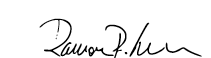
\includegraphics[width=65mm]{figs/logo/assinatura-ramon.png} \\[-4mm]
  \rule[2mm]{70mm}{0.1mm} \\
  \ramon \\[1mm]
  Coordenador do Projeto \\
}

%---------------------------------------------------------------------
\fim



 
\subsection{Abril/2015}
  \subsubsection{Minuta de reunião (16-Abril-2015)}

\begin{tabbing}
  Local \= xxx \kill
  Local \> : LEAD \\
  Data  \> : 16 de Abril de 2015 \\
  Hora  \> : 10:00
\end{tabbing}

%---------------------------------------------------------------------
\participantes{
  \elael,
  \alana,
  \gabriel,
  \julia,
  \ramon,
  \renan.
}

\begin{itemize}
  \item Aprovação da minuta.

  \item Update semanal do Projeto EMMA.
  
  \begin{itemize}
    \item \textbf{\renan.} 
		\begin{itemize}    
			 \item Reportcomp completo.
			 \item Relatório de Eletrônica
			 \item EMMA SOTA 
			
		\end{itemize}
		
		
    \item \textbf{\elael.} 
    		\begin{itemize}    
			 \item Lista de .xml
			 \item Testes executados.
			 \item Proposta Mestrado
			\end{itemize}
					
			
    \item \textbf{\gabriel.} 
    		\begin{itemize}    
			 \item Lista de .xml
			 \item Testes executados.
			 \item Proposta Mestrado
			 \item EMMA SOTA
			\end{itemize}

		 \item \textbf{\julia.} 
    		\begin{itemize}    
			 \item Desenhos de Conceito
			 \item Mestrado
			\end{itemize}

			
  \end{itemize}


  \item Agenda para a próxima reunião:
  \begin{itemize}
    \item Resultado de pesquisas individuais.
    \item Viagem Jirau Abril.
    \item Novas tarefas \& recomendações.
  \end{itemize}

\end{itemize}

\vspace{5mm}%
\parbox[t]{70mm}{
  Aprovado por: \\[5mm]
  \centering
  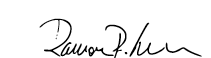
\includegraphics[width=65mm]{figs/logo/assinatura-ramon.png} \\[-4mm]
  \rule[2mm]{70mm}{0.1mm} \\
  \ramon \\[1mm]
  Coordenador do Projeto \\
}

%---------------------------------------------------------------------
\fim
  
\subsection{Maio/2015} 
  \subsubsection{Minuta de reunião (07-Maio-2015)}

\begin{tabbing}
  Local \= xxx \kill
  Local \> : LEAD \\
  Data  \> : 07 de Maio de 2015 \\
  Hora  \> : 10:00
\end{tabbing}

%---------------------------------------------------------------------
\participantes{
  \elael,
  \alana,
  \gabriel,
  \julia,
  \ramon,
  \renan.
}

\textbf{Aprovação da minuta}

\textbf{Update semanal do Projeto EMMA}
  

 \textbf{\alana.} 
	\begin{itemize}
		\item \textbf{Tarefas concluídas:}
			\begin{itemize}    
				\item Diárias e administrativo de viagem.
			\end{itemize}
		
		\item \textbf{Novas tarefas:}
			\begin{itemize} 
				\item Dados ESBR
			\end{itemize}
	\end{itemize}
  
  
\textbf{\renan.} 
	\begin{itemize}
		\item \textbf{Tarefas concluídas:}
			\begin{itemize}    
				\item Analise técnica feita durante a viagem.
			\end{itemize}
		
		\item \textbf{Novas tarefas:}
			\begin{itemize} 
				\item Formalizar análise no EMMA SOTA
				\item conceito escoltilha inferior.
			\end{itemize}
	\end{itemize}
		
\textbf{\elael.} 
	\begin{itemize}
		\item \textbf{Tarefas concluídas:}
			\begin{itemize}    
				\item Ajustes de conceito da escotilha superior.
			\end{itemize}
		
		\item \textbf{Novas tarefas:}
			\begin{itemize} 
				\item Formalizar ajustes no EMMA SOTA
				\item Relatório de viagem Latex.
			\end{itemize}
	\end{itemize}
					
			
   \textbf{\gabriel.} 
	\begin{itemize}
		\item \textbf{Tarefas concluídas:}
			\begin{itemize}    
				\item Analise técnica feita durante a viagem.
			\end{itemize}
		
		\item \textbf{Novas tarefas:}
			\begin{itemize} 
			    \item Conceito Caixa.
				\item Formalizar ajustes no EMMA SOTA
			\end{itemize}
	\end{itemize}

			



\textbf{Agenda para a próxima reunião:}
  \begin{itemize}
    \item Resultado de pesquisas individuais.
    \item Novas tarefas \& recomendações.
  \end{itemize}


\vspace{5mm}%
\parbox[t]{70mm}{
  Aprovado por: \\[5mm]
  \centering
  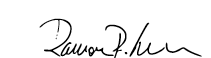
\includegraphics[width=65mm]{figs/logo/assinatura-ramon.png} \\[-4mm]
  \rule[2mm]{70mm}{0.1mm} \\
  \ramon \\[1mm]
  Coordenador do Projeto \\
}

%---------------------------------------------------------------------
\fim
  \subsubsection{Minuta de reunião (14-maio-2015)}

\begin{tabbing}
  Local \= xxx \kill
  Local \> : LEAD \\
  Data  \> : 14 de Maio de 2015 \\
  Hora  \> : 10:00
\end{tabbing}

%---------------------------------------------------------------------
\participantes{
  \elael,
  \alana,
  \gabriel,
  \julia,
  \ramon,
  \renan.
}


\textbf{Aprovação da minuta}

\textbf{Update semanal do Projeto EMMA}
  
\textbf{\renan.} 
	\begin{itemize}
		\item \textbf{Tarefas concluídas:}
			\begin{itemize}    
				\item Fez Apresentação sobre seu conceito Escotilha
     Inferior: questões gerais, pros \& cons, soluções de logística, soluções de
     robótica
			\end{itemize}
		
		\item \textbf{Novas tarefas:}
			\begin{itemize} 
				\item Começar a trabalhar com a questão de reparos de
	turbinas e como determinar a posição do manipulador em relação a pá. 
				\item Análise de Risco.
			\end{itemize}
	\end{itemize}
	
\textbf{\elael.} 
    \begin{itemize}    
		\item \textbf{Tarefas concluídas:}
			\begin{itemize}
				\item Questões comuns do problema.
				\item Consolidar possiveis soluções 
			\end{itemize}
			
		\item \textbf{Novas tarefas:}
			\begin{itemize} 
				\item Calcular base articulada.
				\item Verificar payload.			
			\end{itemize}
	\end{itemize}
	
\textbf{\gabriel.} 
	\begin{itemize}
		\item \textbf{Tarefas concluídas:}
			\begin{itemize}    
				\item Questões comuns do problema.
				\item Consolidar possiveis soluções 
			\end{itemize}
		\item \textbf{Novas tarefas:}
			\begin{itemize}
				\item Calcular base articulada.
				\item Verificar payload.		
			\end{itemize}
	\end{itemize}
	
\textbf{\julia.} 
	\begin{itemize}
		\item \textbf{Tarefas concluídas:}
			\begin{itemize}    
				\item Administrativo Relátorios e Notas.
				\item Tradução para SOTA.
				\item Entrevista com possíveis orientadores.
			\end{itemize}
		\item \textbf{Novas tarefas:}
			\begin{itemize}
				\item Dados ESBR.
				\item Revisão de Proposta.		
			\end{itemize}
	\end{itemize}

%   \item Problemas em aberto:
%   \begin{itemize}
%     \item Procedimento de compras e medidas para as instalações finais do
%     laboratório.
%     \item Opções para a comprar de software, Adobe/ Solid Works/ Live
%     Meeting/Bibliografia
%     \item Fechar orçamento Inventário.
%     \item Criar log para documentar problemas de ROCK/ criar um forum para
%     colaboração (?!)
%     \item Dropbox para compartilhamento de arquivos.
%     \item Viagem ESB/Relatório:
%   \end{itemize}
\textbf{Agenda para a próxima reunião:}
  \begin{itemize}
    \item Resultado de pesquisas individuais.
    \item Viagem Jirau Abril.
    \item Novas tarefas \& recomendações.
  \end{itemize}

\vspace{5mm}%
\parbox[t]{70mm}{
  Aprovado por: \\[5mm]
  \centering
  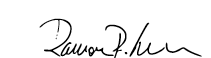
\includegraphics[width=65mm]{figs/logo/assinatura-ramon.png} \\[-4mm]
  \rule[2mm]{70mm}{0.1mm} \\
  \ramon \\[1mm]
  Coordenador do Projeto \\
}

%---------------------------------------------------------------------
\fim
  \subsubsection{Minuta de reunião (21-Maio-2015)}

\begin{tabbing}
  Local \= xxx \kill
  Local \> : LEAD \\
  Data  \> : 21 de Maio de 2015 \\
  Hora  \> : 10:00
\end{tabbing}

%---------------------------------------------------------------------
\participantes{
  \elael,
  \alana,
  \gabriel,
  \julia,
  \ramon,
  \renan.
}

  
\begin{itemize}
  \item Aprovação da minuta.

  \item Update semanal do Projeto EMMA.
  
  
    \item \textbf{\renan.} 
		\begin{itemize}    
			 \item Apresentação conceito Escotilha Inferior
			 \item Correções EMMA SOTA 
			
		\end{itemize}
		
		
    \item \textbf{\elael.} 
    		\begin{itemize}    
			 \item Apresentação conceito Escotilha Superior. 
			 \item Correções EMMA SOTA 
			\end{itemize}
					
			
    \item \textbf{\gabriel.} 
    		\begin{itemize}    
		 \item Apresentação conceito Caixa. 
		 \item Correções EMMA SOTA. 
			\end{itemize}

		 \item \textbf{\julia.} 
    		\begin{itemize}    
			 \item Relatórios ESBR
			 \item PR EMMA/Projeto no Site
			 \item Livro de Atas
		
			\end{itemize}


  \item Agenda para a próxima reunião:
  \begin{itemize}
    \item Resultado de pesquisas individuais.
    \item Novas tarefas \& recomendações.
  \end{itemize}

\end{itemize}

\vspace{5mm}%
\parbox[t]{70mm}{
  Aprovado por: \\[5mm]
  \centering
  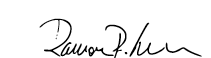
\includegraphics[width=65mm]{figs/logo/assinatura-ramon.png} \\[-4mm]
  \rule[2mm]{70mm}{0.1mm} \\
  \ramon \\[1mm]
  Coordenador do Projeto \\
}

%---------------------------------------------------------------------
\fim
  %---------------------------------------------------------------------
\subsubsection{Minuta de reunião (28-maio-2015)}

\begin{tabbing}
  Local \= xxx \kill
  Local \> : LEAD \\
  Data  \> : 28 de Maio de 2015 \\
  Hora  \> : 10:00
\end{tabbing}

%---------------------------------------------------------------------
\participantes{
  \elael,
  \gabriel,
  \julia,
  \patrick,
  \alana,
  \ramon,
  \renan.
}

\textbf{Aprovação da minuta}

\textbf{Update semanal do Projeto EMMA}
  
\textbf{\renan.} 
	\begin{itemize}
		\item \textbf{Tarefas concluídas:}
			\begin{itemize}    
				\item Ajustes de conceito da escotilha inferior.
			\end{itemize}
		
		\item \textbf{Novas tarefas:}
			\begin{itemize} 
				\item Formalizar ajustes no EMMA SOTA
			\end{itemize}
	\end{itemize}
	
\textbf{\elael.} 
    \begin{itemize}    
		\item \textbf{Tarefas concluídas:}
			\begin{itemize}
				\item Análise de torc e vibração.
				\item Explorou possibilidades para menosr vibração.
				\item Possibilidades relacionadas ao tamanho de braço do robô
			\end{itemize}
			
		\item \textbf{Novas tarefas:}
			\begin{itemize} 
				\item ver com Ramon se será necessário o uso de um 'demper'ou não.
				\item Ver a menos velocidade na qual a base permitirá a continuidade do
				processo de coating.
				\item Frmalizar alterações no SOTA.
			\end{itemize}
	\end{itemize}
	
\textbf{\gabriel.} 
	\begin{itemize}
		\item \textbf{Tarefas concluídas:}
			\begin{itemize}    
				\item Problemas relacionados ao ambiente da unidade geradora.
				\item Ë preciso entender como a curvatura do ambiente pode alterar a
				estabilidade do braço.
			\end{itemize}
		\item \textbf{Novas tarefas:}
			\begin{itemize}
				\item Parafusos nmmagnéticos: qual teria de ser o peso para segurar a base.
				Efeitos colaterais de agua, pressão e deformidade do ambiente.
				\item Frmalizar alterações no SOTA.		
			\end{itemize}
	\end{itemize}
	
\textbf{\julia.} 
	\begin{itemize}
		\item \textbf{Tarefas concluídas:}
			\begin{itemize}    
				\item Administrativo Relátorios e Notas
				\item Mestrado 
			\end{itemize}
		\item \textbf{Novas tarefas:}
			\begin{itemize}
				\item Apresentação EMMA, formalizar o conteúdo do projeto de
				forma clara para divulgação e explicação do projeto.
				\item Vídeo EMMA Aevo.
			\end{itemize}
	\end{itemize}
%   \item Problemas em aberto:
%   \begin{itemize}
%     \item Procedimento de compras e medidas para as instalações finais do
%     laboratório.
%     \item Opções para a comprar de software, Adobe/ Solid Works/ Live
%     Meeting/Bibliografia
%     \item Fechar orçamento Inventário.
%     \item Criar log para documentar problemas de ROCK/ criar um forum para
%     colaboração (?!)
%     \item Dropbox para compartilhamento de arquivos.
%     \item Viagem ESB/Relatório:
%   \end{itemize}

\textbf{Agenda para a próxima reunião:}
	\begin{itemize}
		\item Resultado de pesquisas individuais.
	    \item Viagem Jirau Abril.
	    \item Novas tarefas \& recomendações.
	\end{itemize}


\vspace{5mm}%
\parbox[t]{70mm}{
  Aprovado por: \\[5mm]
  \centering
  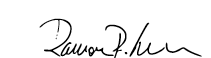
\includegraphics[width=65mm]{figs/logo/assinatura-ramon.png} \\[-4mm]
  \rule[2mm]{70mm}{0.1mm} \\
  \ramon \\[1mm]
  Coordenador do Projeto \\
}

%---------------------------------------------------------------------
\fim


 

\subsection{Junho/2015}
   \subsubsection{Minuta de reunião (11-Junho-2015)}

\begin{tabbing}
  Local \= xxx \kill
  Local \> : LEAD \\
  Data  \> : 11 de Junho de 2015 \\
  Hora  \> : 9:00
\end{tabbing}

%---------------------------------------------------------------------
\participantes{
  \elael,
  \alana,
  \gabriel,
  \julia,
  \ramon,
  \renan.
}

\textbf{Aprovação da minuta}

\textbf{Update semanal do Projeto EMMA}
   
\textbf{\julia.} 
	\begin{itemize}
		\item \textbf{Tarefas concluídas:}
			\begin{itemize}    
				\item Apresentação EMMA.
				\item ADM/ Documentos /Viagem
			\end{itemize}
		
		\item \textbf{Novas tarefas:}
			\begin{itemize} 
				\item Atualizar documentação.
				\item Finalizar apresentação.
				\item Mestrado: questões relaciondas ao tema de controle de missão
				robótica.
			\end{itemize}
	\end{itemize}
					
		
\textbf{\elael.} 
	\begin{itemize}
		\item \textbf{Tarefas concluídas:}
			\begin{itemize}    
				\item Checou menor velocidade que possível para a base que permite a
				aplicação continua de coating.
				\item \item Calculou valores de torc.
			\end{itemize}
		
		\item \textbf{Novas tarefas:}
			\begin{itemize} 
				\item Formalizar ajustes no EMMA SOTA.
				\item Estudo sobre Shutter.
				\item Auxiliar estevão no desenho da Base.
			\end{itemize}
	\end{itemize}
					
\textbf{\gabriel.} 
	\begin{itemize}
		\item \textbf{Tarefas concluídas:}
			\begin{itemize}    
				\item analisouparafusos magnéticos.
				\item Modelo 3D em OpenRave.
			\end{itemize}
		
		\item \textbf{Novas tarefas:}
			\begin{itemize} 
				\item Formalizar ajustes no EMMA SOTA.
				\item Checar viabilidade de operaçào no espaço atrás das pás.
				\item Verificar manipuladores.
			\end{itemize}
	\end{itemize}
					
			
   \textbf{\estevão.} 
	\begin{itemize}
		\item \textbf{Tarefas concluídas:}
			\begin{itemize}    
				\item Trabalhou no modelo 3D da unidade geradora.
			\end{itemize}
		
		\item \textbf{Novas tarefas:}
			\begin{itemize} 
			    \item Terminar modelo 3D da unidade geradora.
				\item Desenho da base com Elael.
			\end{itemize}
	\end{itemize}

			



\textbf{Agenda para a próxima reunião:}
  \begin{itemize}
    \item Resultado de pesquisas individuais.
    \item Novas tarefas \& recomendações.
  \end{itemize}


\vspace{5mm}%
\parbox[t]{70mm}{
  Aprovado por: \\[5mm]
  \centering
  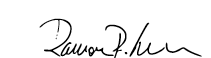
\includegraphics[width=65mm]{figs/logo/assinatura-ramon.png} \\[-4mm]
  \rule[2mm]{70mm}{0.1mm} \\
  \ramon \\[1mm]
  Coordenador do Projeto \\
}

%---------------------------------------------------------------------
\fim
   \subsubsection{Minuta de reunião (17-Junho-2015)}

\begin{tabbing}
  Local \= xxx \kill
  Local \> : LEAD \\
  Data  \> : 17 de Junho de 2015 \\
  Hora  \> : 13:00
\end{tabbing}

%---------------------------------------------------------------------
\participantes{
  \elael,
  \gabriel,
  \julia,
  \ramon.
}

\textbf{Aprovação da minuta}

\textbf{Update semanal do Projeto EMMA}
  
		
\textbf{\elael.} 
	\begin{itemize}
		\item \textbf{Tarefas concluídas:}
			\begin{itemize}    
				\item Estudo do Shutter: ainda espera info da Rijeza com valores
				relacionados a chama (trabalhou com estimativas árbitrárias que nos foram
				dadas anteriormente 3mm/ chama 3mil graus/ 230 mm).
				\item Identificou a classe de materiais (cerâmicas) de resistência para
				altas temperaturas.
				\item Abrir novas possibilidades para o design do shutter.
				\item Auxiliou estevão no elaboração do desenho da base.
			\end{itemize}
		
		\item \textbf{Novas tarefas:}
			\begin{itemize} 
				\item Formalizar ajustes no EMMA SOTA
				\item Atualizar estudo do 'Shutter'com numeros da Rijeza.
				\item Esboço do Shutter com Estevão.
				\item analizar shadow plates.
			\end{itemize}
	\end{itemize}
					
			
   \textbf{\gabriel.} 
	\begin{itemize}
		\item \textbf{Tarefas concluídas:}
			\begin{itemize}    
				\item workspace availability: KUKA 30L16 não é compatível com o ambiente
				(usou 45 graus como referência.) Maniulador  KUKA com 3m de alcance 30 L16,
				para frente da pá funciona bem, porém atras da pa fica incompatível com o
				espaço que temos na unidade geradora.
				\item KUKA KR30 bugado no openRave.
				\item Criou modelo simplificado com cilindros para facilitar KR30, mas ainda
				não acertou todos os eixos, simulação em processo de refinamento.
			\end{itemize}
		
		\item \textbf{Novas tarefas:}
			\begin{itemize} 
			    \item Manipuladores: Verificar modelo novo do motoman, 8 graus de
			    liberdade
			    \item Refinar simulação para incluir qualquer robô.
				\item Formalizar ajustes no EMMA SOTA.
			\end{itemize}
	\end{itemize}
	
	   \textbf{\julia.} 
	\begin{itemize}
		\item \textbf{Tarefas concluídas:}
			\begin{itemize}    
				\item Apresentação de projeto com conteúdo final para feedback de equipe, 
				Ramon e Patrick.
				\item Administrativo (seguro de vida, iniciação científica)
				\item Documentação de projeto atualizada.
			\end{itemize}
		
		\item \textbf{Novas tarefas:}
			\begin{itemize} 
			    \item Assimilar feedback de orientadora na proposta de mestrado
				\item Apresentação coordenada para viagem.
			\end{itemize}
	\end{itemize}

  \textbf{\estevão.} 
	\begin{itemize}
		\item \textbf{Tarefas concluídas:}
			\begin{itemize}    
				\item Elaborou conceito da base com Ramon, desenho em andamento.
				\item Concluiu desenho da unidade geradora.
			\end{itemize}
		
		\item \textbf{Novas tarefas:}
			\begin{itemize} 
			    \item Esboço do shutter.
			    \item Desenho da base.
			\end{itemize}
	\end{itemize}
			



\textbf{Agenda para a próxima reunião:}
  \begin{itemize}
    \item Solução é formada por: base totalmente retrátil + manipulador KUKA
    Lightweight LB820 + Shutter.
    \item Novas tarefas \& recomendações.
  \end{itemize}


\vspace{5mm}%
\parbox[t]{70mm}{
  Aprovado por: \\[5mm]
  \centering
  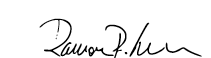
\includegraphics[width=65mm]{figs/logo/assinatura-ramon.png} \\[-4mm]
  \rule[2mm]{70mm}{0.1mm} \\
  \ramon \\[1mm]
  Coordenador do Projeto \\
}

%---------------------------------------------------------------------
\fim
   \subsubsection{Minuta de reunião (24-Junho-2015)}

\begin{tabbing}
  Local \= xxx \kill
  Local \> : LEAD \\
  Data  \> : 24 de Junho de 2015 \\
  Hora  \> : 13:00
\end{tabbing}

%---------------------------------------------------------------------
\participantes{
  \elael,
  \gabriel,
  \julia,
  \renan,
  \alana,
  \estevão,
  \ramon.
}

\textbf{Aprovação da minuta}

\textbf{Update semanal do Projeto EMMA}
  
		
\textbf{\elael.} 
	\begin{itemize}
		\item \textbf{Tarefas concluídas:}
			\begin{itemize}    
				\item Análise do Shutter em andamento com novos números Rijeza.
				\item Análise de material de alta resistência. 
			\end{itemize}
		
		\item \textbf{Novas tarefas:}
			\begin{itemize} 
				\item SOTA: finalizar conceito para deadline de quarta-feira 
				\item Cerâmicas de compressão: descobrir o material que a Rijeza usa.
				\item Email Darlan: Informação sobre a chama e pistola de coating.
			\end{itemize}
	\end{itemize}
	
	\textbf{\renan.} 
	\begin{itemize}
		\item \textbf{Novas tarefas:}
			\begin{itemize} 
				\item Se unir a Gabriel para finalizar a workspace analysis.
				\item Formalizar conclusões no SOTA para deadline.
			\end{itemize}
	\end{itemize}
					
			
   \textbf{\gabriel.} 
	\begin{itemize}
		\item \textbf{Tarefas concluídas:}
			\begin{itemize}    
				\item Bugs no workspace analysis resolvidos.
				\item Análise motoman em andamento.
			\end{itemize}
		
		\item \textbf{Novas tarefas:}
			\begin{itemize} 
			    \item Manipuladores: Verificar modelo novo do motoman, 8 graus de
			    liberdade.
			    \item Resolver 'colisions issues' Open Rave.
				\item Adicionar conclusões no SOTA.
			\end{itemize}
	\end{itemize}
	
	   \textbf{\julia.} 
	\begin{itemize}
		\item \textbf{Tarefas concluídas:}
			\begin{itemize}    
				\item Apresentação
				\item Logo do Projeto EMMA
				\item Documentação de projeto atualizada.
			\end{itemize}
		
		\item \textbf{Novas tarefas:}
			\begin{itemize} 
			    \item Revisão Proposta com Patrick.
			    \item Apresentação EMMA. 
			    \item Cotações viagens.
			\end{itemize}
	\end{itemize}

  \textbf{\estevão.} 
	\begin{itemize}
		\item \textbf{Tarefas concluídas:}
			\begin{itemize}    
				\item Slides com SolidWorks da base para apresentação adicionados.
			\end{itemize}
		
		\item \textbf{Novas tarefas:}
			\begin{itemize} 
			    \item Continuar esboço do shutter.
			    \item Formalizar trabalho de mecânica no SOTA.
			\end{itemize}
	\end{itemize}
			



\textbf{Agenda para a próxima reunião:}
  \begin{itemize}
    \item Novas tarefas \& recomendações.
  \end{itemize}


\vspace{5mm}%
\parbox[t]{70mm}{
  Aprovado por: \\[5mm]
  \centering
  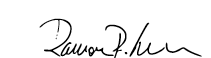
\includegraphics[width=65mm]{figs/logo/assinatura-ramon.png} \\[-4mm]
  \rule[2mm]{70mm}{0.1mm} \\
  \ramon \\[1mm]
  Coordenador do Projeto \\
}

%---------------------------------------------------------------------
\fim


\subsection{Julho/2015}
    \subsubsection{Minuta de reunião (01-Julho-2015)}

\begin{tabbing}
  Local \= xxx \kill
  Local \> : LEAD \\
  Data  \> : 01 de Julho de 2015 \\
  Hora  \> : 13:00
\end{tabbing}

%---------------------------------------------------------------------
\participantes{
  \elael,
  \alana,
  \gabriel,
  \julia,
  \ramon,
  \renan.
}

\textbf{Aprovação da minuta}

\textbf{Update semanal do Projeto EMMA}

\textbf{Considerações Gerais EMMA:}
  \begin{itemize}
    \item Contratações previstas: 1 engenheiro de software, 1 engenheiro de
    eletrônica e um aluno de mestrado de controle.
    \item Primeiro Objetivo do quadrimestre: definir a solução detalhada.
    Análise de riscos e benefícios.
    \item Segundo Objetivo do Quadrimentre: Determinar a relação de posição do
    braço robótico e do ambiente.
    \item Terceiro Objetivo do Quadrimentre: elaboração de tarefas do robô em
    preparo para arquitetura de interface.
  \end{itemize}
  
  
\textbf{\renan.} 
	\begin{itemize}
		\item \textbf{Tarefas concluídas:}
			\begin{itemize}    
				\item SOTA.
			\end{itemize}
		
		\item \textbf{Novas tarefas:}
			\begin{itemize} 
				\item Detalhes do acesso do robô na escotilha inferior.
				\item Apresentação.
			\end{itemize}
	\end{itemize}
		
\textbf{\elael.} 
	\begin{itemize}
		\item \textbf{Tarefas concluídas:}
			\begin{itemize}    
				\item SOTA
			\end{itemize}
		
		\item \textbf{Novas tarefas:}
			\begin{itemize} 
				\item Pesquisar sensores. Localização e Octomap para ajudar no processo de
				de calibração do braço Robótico.
				\item Mapeamento de tarefas do robô para interface de usuário.
			\end{itemize}
	\end{itemize}
					
			
   \textbf{\gabriel.} 
	\begin{itemize}
		\item \textbf{Tarefas concluídas:}
			\begin{itemize}    
				\item SOTA.
			\end{itemize}
		
		\item \textbf{Novas tarefas:}
			\begin{itemize} 
			    \item Procurar OpenSource para auxiliar no processo de calibração do
			    braço robótico.
				\item Mapeamento de tarefas do robô para interface de usuário.
			\end{itemize}
	\end{itemize}

			
		
   \textbf{\estevão.} 
	\begin{itemize}
		\item \textbf{Tarefas concluídas:}
			\begin{itemize}    
				\item SOTA.
			\end{itemize}
		
		\item \textbf{Novas tarefas:}
			\begin{itemize} 
			    \item Definir conceito da base para suporte de manipulador na entrada da
			    escotilha inferior.
			\end{itemize}
	\end{itemize}
	
		
   \textbf{\estevão.} 
	\begin{itemize}
		\item \textbf{Tarefas concluídas:}
			\begin{itemize}    
				\item Apresentação
			\end{itemize}
		
		\item \textbf{Novas tarefas:}
			\begin{itemize} 
			    \item Estudo das tarefas do robô e seu mapeamento para a construção da
			    interface de usuário.
			\end{itemize}
	\end{itemize}

			



\textbf{Agenda para a próxima reunião:}
  \begin{itemize}
    \item Resultado de pesquisas individuais.
    \item Novas tarefas \& recomendações.
  \end{itemize}


\vspace{5mm}%
\parbox[t]{70mm}{
  Aprovado por: \\[5mm]
  \centering
  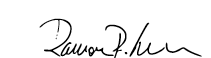
\includegraphics[width=65mm]{figs/logo/assinatura-ramon.png} \\[-4mm]
  \rule[2mm]{70mm}{0.1mm} \\
  \ramon \\[1mm]
  Coordenador do Projeto \\
}

%---------------------------------------------------------------------
\fim
    \subsubsection{Minuta de reunião (08-Julho-2015)}

\begin{tabbing}
  Local \= xxx \kill
  Local \> : LEAD \\
  Data  \> : 08 de Julho de 2015 \\
  Hora  \> : 13:00
\end{tabbing}

%---------------------------------------------------------------------
\participantes{
  \elael,
  \alana,
  \gabriel,
  \julia,
  \ramon,
  \renan.
}

\textbf{Aprovação da minuta}

\textbf{Update semanal do Projeto EMMA}

  
\textbf{\renan.} 
	\begin{itemize}
		\item \textbf{Tarefas concluídas:}
			\begin{itemize}    
				\item Pesquisa de braços robóticos com boa relaçào entre peso e alcance.
				KUKA KR10 com 6 graus de liberdade e 10kg de payload.
				\item Apresentação para Rijeza em Porto Alegre.
			\end{itemize}
		
		\item \textbf{Novas tarefas:}
			\begin{itemize} 
				\item Metodologia de análise para braços robóticos.
			\end{itemize}
	\end{itemize}
		
\textbf{\elael.} 
	\begin{itemize}
		\item \textbf{Tarefas concluídas:}
			\begin{itemize}    
				\item Estado da Arte para calibração de braços robóticos.
				\item Encontrou uma solução para reparo que menciona localização por 3D. 
			\end{itemize}
		
		\item \textbf{Novas tarefas:}
			\begin{itemize} 
				\item Encontrar uma forma de reduzir o peso dos cabos.(email Darlan)
			\end{itemize}
	\end{itemize}
					
			
   \textbf{\gabriel.} 
	\begin{itemize}
		\item \textbf{Tarefas concluídas:}
			\begin{itemize}    
				\item Estudo sobre sensores e seus respectivos drivers, pontos fracos e
				fortes, como se enquadrariam em nossa solução.  
			\end{itemize}
		
		\item \textbf{Novas tarefas:}
			\begin{itemize} 
			    \item Pesquisar Sensores 1D
			    \item Auxiliar workspace analisys de Rena e Estevão com Open Rave. 
			\end{itemize}
	\end{itemize}

			
\textbf{\estevão.} 
	\begin{itemize}
		\item \textbf{Tarefas concluídas:}
			\begin{itemize}    
				\item Pesquisa de braços robóticos com boa relaçào entre peso e alcance.
				KUKA KR10 com 6 graus de liberdade e 10kg de payload.
				\item Trabalhou com a hipótese de 4 posições para cobrir a pá.
			\end{itemize}
		
		\item \textbf{Novas tarefas:}
			\begin{itemize} 
				\item Metodologia de análise para braços robóticos.
				\item Estudar qual o alcance e graus de liberdade pra cobrir a pá.
			\end{itemize}
	\end{itemize}
	
		
   \textbf{\julia.} 
	\begin{itemize}
		\item \textbf{Tarefas concluídas:}
			\begin{itemize}    
				\item Estudo das tarefas do robô e seu mapeamento para a construção da
			    interface de usuário.
			    \item Apresentou organograma das tarefas do Robô com descrição de
				atividades da interface do usuário.
			\end{itemize}
		
		\item \textbf{Novas tarefas:}
			\begin{itemize} 
			 \item Fluxograma, pesquisar para descrever em fluxograma completo os
			 processos relacionados a calibração, Reparo, Metalização e Jatemaneto
			 \item Distinguir e detalhar cada processo de tarefas. 
			\end{itemize}
	\end{itemize}

			



\textbf{Agenda para a próxima reunião:}
  \begin{itemize}
    \item Resultado de pesquisas individuais.
    \item Novas tarefas \& recomendações.
  \end{itemize}


\vspace{5mm}%
\parbox[t]{70mm}{
  Aprovado por: \\[5mm]
  \centering
  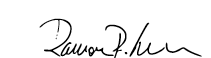
\includegraphics[width=65mm]{figs/logo/assinatura-ramon.png} \\[-4mm]
  \rule[2mm]{70mm}{0.1mm} \\
  \ramon \\[1mm]
  Coordenador do Projeto \\
}

%---------------------------------------------------------------------
\fim 
    \subsubsection{Minuta de reunião (15-Julho-2015)}

\begin{tabbing}
  Local \= xxx \kill
  Local \> : LEAD \\
  Data  \> : 15 de Julho de 2015 \\
  Hora  \> : 13:00
\end{tabbing}

%---------------------------------------------------------------------
\participantes{
  \elael,
  \alana,
  \gabriel,
  \julia,
  \ramon,
  \renan.
}

\textbf{Aprovação da minuta}

\textbf{Update semanal do Projeto EMMA}

  
\textbf{\renan.} 
	\begin{itemize}
		\item \textbf{Tarefas concluídas:}
			\begin{itemize}    
				\item Repasse do relatório da viagem a Rijeza.
			\end{itemize}
		
		\item \textbf{Novas tarefas:}
			\begin{itemize} 
				\item Dar continuidade a análise de pás com Estevão.
				\item Formalizar descobertas de Porto Alegre, e dar início a um novo
				Journal.
			\end{itemize}
	\end{itemize}
		
\textbf{\elael.} 
	\begin{itemize}
		\item \textbf{Tarefas concluídas:}
			\begin{itemize}    
				\item Pesquisa de Sensores.
			\end{itemize}
		
		\item \textbf{Novas tarefas:}
			\begin{itemize} 
				\item Formalizar Pesquisa de Sensores.
			\end{itemize}
	\end{itemize}
					
			
   \textbf{\gabriel.} 
	\begin{itemize}
		\item \textbf{Tarefas concluídas:}
			\begin{itemize}    
				\item Formalizou pesquisa de Sensores de alta precisão com pros e cons:
				Pros: sensores não são 3d e sim fechos de laser com um espelho giratório e
				um PanTilt que varre o ambiente.
				Cons: Tais sensores demoram muito para fazer a varredura completa.
			\end{itemize}
		
	\end{itemize}

			
\textbf{\estevão.} 
	\begin{itemize}
		\item \textbf{Tarefas concluídas:}
			\begin{itemize}    
				\item Metodologia criada: malha de pontos, rotina que identifica o
				manipulador específico que atende aos parâmetros do projeto. Os
				manipuladores pesquisados estão sendo adicionados de acordo.
				\item Análise cinemática e dinâmica com OpenRave e MathLab para simulação
				dinâmica.
			\end{itemize}
		
		\item \textbf{Novas tarefas:}
			\begin{itemize} 
				\item Produzor gráfico para pá robótica.
				\item Maquete de braço.
				\item Opções de estagiário.
			\end{itemize}
	\end{itemize}
	
		
   \textbf{\julia.} 
	\begin{itemize}
		\item \textbf{Tarefas concluídas:}
			\begin{itemize}    
				\item Fluxograma com tarefas do robô descritas
			    \item Estudo de artigos para pesquisa de mapping e visualização de data.
			\end{itemize}
		
		\item \textbf{Novas tarefas:}
			\begin{itemize} 
			 \item Fluxograma Macro
			 \item Formalizar pesquisa de Mapping.
			 \item Entregar proposta revisada
			\end{itemize}
	\end{itemize}

			



\textbf{Agenda para a próxima reunião:}
  \begin{itemize}
    \item Resultado de pesquisas individuais.
    \item Novas tarefas \& recomendações.
  \end{itemize}


\vspace{5mm}%
\parbox[t]{70mm}{
  Aprovado por: \\[5mm]
  \centering
  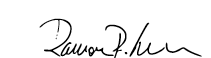
\includegraphics[width=65mm]{figs/logo/assinatura-ramon.png} \\[-4mm]
  \rule[2mm]{70mm}{0.1mm} \\
  \ramon \\[1mm]
  Coordenador do Projeto \\
}

%---------------------------------------------------------------------
\fim
    \subsubsection{Minuta de reunião (22-Julho-2015)}

\begin{tabbing}
  Local \= xxx \kill
  Local \> : LEAD \\
  Data  \> : 22 de Julho de 2015 \\
  Hora  \> : 13:00
\end{tabbing}

%---------------------------------------------------------------------
\participantes{
  \alana,
  \julia,
  \estevão,
  \ramon,
  \renan.
}

\textbf{Aprovação da minuta}

\textbf{Update semanal do Projeto EMMA}

  
\textbf{\renan.} 
	\begin{itemize}
		\item \textbf{Tarefas concluídas:}
			\begin{itemize}    
				\item Apresentação da Solução pela escotilha inferior.
 				\item Pesquisa de Manipuladores: comparação de modelos KUKA e
 				MOTOMAN, peso, alcance, menores distâncias, posições
 				em relação a pá, todas formalizadas em uma tabela.
 				\item Estudo de cinemática e colisões.
			\end{itemize}
		
		\item \textbf{Novas tarefas:}
			\begin{itemize} 
				\item Adicionar o KUKA lightweight a pesquisa, approach geométrico, fotos e
				legendas. 
				\item Adicionar causa de recusa.
			\end{itemize}
	\end{itemize}

			
\textbf{\estevão.} 
	\begin{itemize}
		\item \textbf{Tarefas concluídas:}
			\begin{itemize}    
				\item Desenhos da base em trilho para escotilha inferior, com ambos
				manipuladores, Motoman e KUKA anexado a apresentação do Renan.
			\end{itemize}
		
		\item \textbf{Novas tarefas:}
			\begin{itemize} 
				\item Estudo com base e trilho para escotilha inferior com ambas
				manipuladores KUKA e Motoman.
				\item Fechar de estagiário.
			\end{itemize}
	\end{itemize}
	
		
   \textbf{\julia.} 
	\begin{itemize}
		\item \textbf{Tarefas concluídas:}
			\begin{itemize}    
				\item Proposta de Mestrado Final
				\item Apresentação de Resumo dos Artigos
			\end{itemize}
		
		\item \textbf{Novas tarefas:}
			\begin{itemize} 
			 \item Pesquisa: Estado da Arte para Interfaces Gráficas para Manipuladores.
			\end{itemize}
	\end{itemize}


\textbf{Agenda para a próxima reunião:}
  \begin{itemize}
    \item Resultado de pesquisas individuais.
    \item Novas tarefas \& recomendações.
  \end{itemize}


\vspace{5mm}%
\parbox[t]{70mm}{
  Aprovado por: \\[5mm]
  \centering
  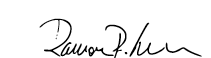
\includegraphics[width=65mm]{figs/logo/assinatura-ramon.png} \\[-4mm]
  \rule[2mm]{70mm}{0.1mm} \\
  \ramon \\[1mm]
  Coordenador do Projeto \\
}

%---------------------------------------------------------------------
\fim
    \subsubsection{Minuta de reunião (29-Julho-2015)}

\begin{tabbing}
  Local \= xxx \kill
  Local \> : LEAD \\
  Data  \> : 29 de Julho de 2015 \\
  Hora  \> : 13:00
\end{tabbing}

%---------------------------------------------------------------------
\participantes{
  \alana,
  \julia,
  \estevão,
  \ramon,
  \renan.
}

\textbf{Aprovação da minuta}

\textbf{Update semanal do Projeto EMMA}

  
\textbf{\renan.} 
	\begin{itemize}
		\item \textbf{Tarefas concluídas:}
			\begin{itemize}    
				\item Apresentação da Solução pela escotilha inferior.
 				\item Formalizou KUKA lightweight na pesquisa, com desenhos novos do
 				Estevão.
 				\item Apresentou tabela com todas as possíveis intituições para
 				publicações no setor de energia.
			\end{itemize}
		
		\item \textbf{Novas tarefas:}
			\begin{itemize} 
				\item Formalizar avanços da pesquisa de cinemática no Journal.
				\item Revisar SOTA e definir onde vamos publicar com Ramon.
				\item Decidir qual Robô vamos comprar, entrar em contato com fabricante.
			\end{itemize}
	\end{itemize}

			
\textbf{\estevão.} 
	\begin{itemize}
		\item \textbf{Tarefas concluídas:}
			\begin{itemize}    
				\item Desenhos da base em trilho para escotilha inferior, com ambos
				manipuladores, Motoman e KUKA anexado a apresentação do Renan.
			\end{itemize}
		
		\item \textbf{Novas tarefas:}
			\begin{itemize} 
				\item Desenhar base flat com os pontos de solda.
				\item Maquete usando impressora 3D. (ver com alana para incluir em material
				de consumo)
				\item Fazer esboço com 1 grau de liberdade mais movimentação da pá.
				\item Comprar base magnética para testar pontos de fixação.
			\end{itemize}
	\end{itemize}
	
		
   \textbf{\julia.} 
	\begin{itemize}
		\item \textbf{Tarefas concluídas:}
			\begin{itemize}    
				\item Apresentação Estado da Arte em maniouladores para Robôs.
			\end{itemize}
		
		\item \textbf{Novas tarefas:}
			\begin{itemize} 
			 \item Continuar pesquisa: adicionar questões de IHC e Design de interfaces.
			\end{itemize}
	\end{itemize}


\textbf{Agenda para a próxima reunião:}
  \begin{itemize}
    \item Resultado de pesquisas individuais. 
    \item Novas tarefas \& recomendações.
  \end{itemize}


\vspace{5mm}%
\parbox[t]{70mm}{
  Aprovado por: \\[5mm]
  \centering
  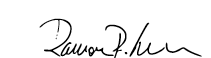
\includegraphics[width=65mm]{figs/logo/assinatura-ramon.png} \\[-4mm]
  \rule[2mm]{70mm}{0.1mm} \\
  \ramon \\[1mm]
  Coordenador do Projeto \\
}

%---------------------------------------------------------------------
\fim     
    
\subsection{Agosto/2015}
   \subsubsection{Minuta de reunião (12-Agosto-2015)}

\begin{tabbing}
  Local \= xxx \kill
  Local \> : LEAD \\
  Data  \> : 12 de Agosto de 2015 \\
  Hora  \> : 13:00
\end{tabbing}

%---------------------------------------------------------------------
\participantes{
  \elael,
  \alana,
  \gabriel,
  \julia,
  \estevão,
  \renan.
}

\textbf{Aprovação da minuta}

\textbf{Update semanal do Projeto EMMA}

\textbf{\alana.} 
	\begin{itemize}
		\item \textbf{Tarefas concluídas:}
			\begin{itemize}    
				\item Entregas de documentos auditoria.
				\item Planilha e gastos versus atividades.
			\end{itemize}
		
		\item \textbf{Novas tarefas:}
			\begin{itemize} 
				\item Planilha de prestação de contas. 
			\end{itemize}
	\end{itemize}   							

\textbf{\elael.} 
	\begin{itemize}
		\item \textbf{Tarefas concluídas:}
			\begin{itemize}    
				\item Pesquisa de sensores de point laser. 
			\end{itemize}
		
		\item \textbf{Novas tarefas:}
			\begin{itemize} 
				\item Escolher equipamento para calibração.
				\item Começar mexer com o LMS111 Laser scan. 
			\end{itemize}
	\end{itemize}
	
	\textbf{\julia.} 
	\begin{itemize}
		\item \textbf{Tarefas concluídas:}
			\begin{itemize}    
				\item ADM: Passagens e viagem CITENEL
				\item Acerto de possível co-orientadora para mestrado, ajustes na proposta
				de acordo.
			\end{itemize}
		
		\item \textbf{Novas tarefas:}
			\begin{itemize} 
				\item: Apresentação de Metodologia para o design de interface do software do
				projeto.
			\end{itemize}
	\end{itemize}
					
\textbf{\gabriel.} 
	\begin{itemize}
		\item \textbf{Tarefas concluídas:}
			\begin{itemize}    
				\item Pesquisa de Sensores 2D.
			\end{itemize}
		
		\item \textbf{Novas tarefas:}
			\begin{itemize} 
				\item Escolher equipamento para calibração.
				\item Começar mexer com o LMS111 Laser scan. 
				\item Reuniões com diferentes fornecedores de sensores. (NIKON, FARO,
				LEICA, CIK).
			\end{itemize}
	\end{itemize}
					
			
   \textbf{\estevão.} 
	\begin{itemize}
		\item \textbf{Tarefas concluídas:}
			\begin{itemize}    
				\item Apresentação sobre Cinemática dos braços robóticos possíveis, 
				tabela comparativa, pontos fortes e fracos.
				\item Estudo de diferentes supporte para a solução da escotilha inferior,
				desenhos de solid works.
			\end{itemize}
		
		\item \textbf{Novas tarefas:}
			\begin{itemize} 
			    \item Desenho Motoman sem graus de liberdade.
			    \item Maquete: Possibilidades de execução junto a Escola de Belas Artes
			    (EBA) e justificativa técnica para rúbrica de serviços.
			\end{itemize}
	\end{itemize}

			
   \textbf{\renan.} 
	\begin{itemize}
		\item \textbf{Tarefas concluídas:}
			\begin{itemize}    
				\item Apresentação sobre Cinemática dos braços robóticos possíveis, 
				tabela comparativa, pontos fortes e fracos.
				\item Estudo de diferentes supporte para a solução da escotilha inferior,
				calculos e comparação de áreas de coating possíveis.
			\end{itemize}
		
		\item \textbf{Novas tarefas:}
			\begin{itemize} 
			    \item Checar os alcance dos braços escolhidos em 30 graus.
			\end{itemize}
	\end{itemize}		



\textbf{Agenda para a próxima reunião:}
  \begin{itemize}
    \item Resultado de pesquisas individuais.
    \item Novas tarefas \& recomendações.
  \end{itemize}


\vspace{5mm}%
\parbox[t]{70mm}{
  Aprovado por: \\[5mm]
  \centering
  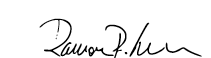
\includegraphics[width=65mm]{figs/logo/assinatura-ramon.png} \\[-4mm]
  \rule[2mm]{70mm}{0.1mm} \\
  \ramon \\[1mm]
  Coordenador do Projeto \\
}

%---------------------------------------------------------------------
\fim
   \subsubsection{Minuta de reunião (19-Agosto-2015)}

\begin{tabbing}
  Local \= xxx \kill
  Local \> : LEAD \\
  Data  \> : 19 de Agosto de 2015 \\
  Hora  \> : 13:00
\end{tabbing}

%---------------------------------------------------------------------
\participantes{
  \gabriel,
  \julia,
  \estevão,
  \ramon.

}

\textbf{Aprovação da minuta}

\textbf{Update semanal do Projeto EMMA}
   							
					
\textbf{\gabriel.} 
	\begin{itemize}
		\item Escolher equipamento para calibração.
				\item Usou ROS e ROCK com LMS111 Laser scan, porém nenhum funcionou bem.
				\item Reunião Nikon Metrology: eles podem nos fornecer a solução completa
				para calibração, porém precisam de pelo menos 2.5 metros de distância
				dos alvos para fazerem a leitura.
				\item Reunião com FARO essa semana.
			\end{itemize}
		
		\item \textbf{Novas tarefas:}
			\begin{itemize} 
				\item Reunião com FARO.
				\item Implementar o driver do ROS no ROCK para fazer o Laser Scan LMS111
				funcionar bem.
			\end{itemize}

					
			
   \textbf{\estevão.} 
	\begin{itemize}
		\item \textbf{Tarefas concluídas:}
			\begin{itemize}    
				\item Desenhou o modelo da maquete, pediu cotações para as peças que
				queremos imprimir 3D. Apenas a pá sairia entre 5 e 7 mil reais, resultando
				em um valor muito alto. 
				\item Conversou com prossor da EBA sobre a possiblidades de fazer a maquete.
				\item Desenho dos braços sem os graus de liberdade apresentou problema co
				relação ao acesso dos cabos por cima quando o robô estiver na frente da pá.
				
			\end{itemize}
		
		\item \textbf{Novas tarefas:}
			\begin{itemize} 
			    \item Continuar estudo da solução da escotilha inferior com Renan.
			    \item Fazer estudo se teremos de conectar e desconetar os cabos toda vez
			    que tivermos de girar o rotor.
				\item Atualização do modelo maquete.
			    \item Solid works: Desnehar o lipe da pá.
			\end{itemize}
	\end{itemize}

	  \textbf{\Renan.} 
	\begin{itemize}
		\item \textbf{Tarefas concluídas:}
			\begin{itemize}    
				\item Fez um estudo da dos tolerancia no end effector. 
			\end{itemize}
		
		\item \textbf{Novas tarefas:}
			\begin{itemize} 
			    \item Formalizar no SOTA. 
			\end{itemize}
	\end{itemize}		
			
			
   \textbf{\Julia.} 
	\begin{itemize}
		\item \textbf{Tarefas concluídas:}
			\begin{itemize}    
				\item Proposta de Mestrado para PUC e UFRJ.
				\item Metodologia de Interface Gráfica do controle de missão do projeto.
			\end{itemize}
		
		\item \textbf{Novas tarefas:}
			\begin{itemize} 
			    \item Continuar trabalho de metodologia e apresenta-los para os
			    integrantes da equipe que estavam no congresso CITENEL.
			    \item Buscar Engenheiro de software para o projeto. (processo de
			    seleção a ser discutido).
			\end{itemize}
	\end{itemize}		



\textbf{Agenda para a próxima reunião:}
  \begin{itemize}
    \item Resultado de pesquisas individuais.
    \item Novas tarefas \& recomendações.
  \end{itemize}


\vspace{5mm}%
\parbox[t]{70mm}{
  Aprovado por: \\[5mm]
  \centering
  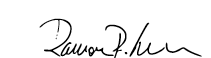
\includegraphics[width=65mm]{figs/logo/assinatura-ramon.png} \\[-4mm]
  \rule[2mm]{70mm}{0.1mm} \\
  \ramon \\[1mm]
  Coordenador do Projeto \\
}

%---------------------------------------------------------------------
\fim
   \subsubsection{Minuta de reunião (26-Agosto-2015)}

\begin{tabbing}
  Local \= xxx \kill
  Local \> : LEAD \\
  Data  \> : 26 de Agosto de 2015 \\
  Hora  \> : 13:00
\end{tabbing}

%---------------------------------------------------------------------
\participantes{
  \gabriel,
  \julia,
  \estevão,
  \elael,
  \renan,
  \ramon.

}

\textbf{Aprovação da minuta}

\textbf{Update semanal do Projeto EMMA}
   							
\textbf{\alana.} 
	\begin{itemize}
		\item \textbf{Tarefas concluídas:}
			\begin{itemize}    
				\item Prestação de contas.
			\end{itemize}
		
		\item \textbf{Novas tarefas:}
			\begin{itemize} 
				\item Relatório de Auditoria.
				\item Ofícios.
			\end{itemize}
	\end{itemize}   		
						
\textbf{\gabriel.} 
	\begin{itemize}
			\item Resumiu suas reuniões com fornecedores de sensores, seu preços,
			cacidades e aplicações para o projeto.
			\item Implementação driver ROS para ROCK do laser scan em progresso.
			\end{itemize}
		
		\item \textbf{Novas tarefas:}
			\begin{itemize} 
				\item Incluir novas cotações para sensores Velodine e Leica.
				\item Continuar implementaçãod do driver do laser scan.
				\item Estudar possibilidades para Point Cloud Alignment.
			\end{itemize}

					
			
   \textbf{\estevão.} 
	\begin{itemize}
		\item \textbf{Tarefas concluídas:}
			\begin{itemize}    
				\item Apresentou com Renan dados para solução da escotilha inferior sem
				graus de liberdade.
				\item Conseguiu dois orçamentos maquete.
				
			\end{itemize}
		
		\item \textbf{Novas tarefas:}
			\begin{itemize} 
			    \item Conceito sobre solução de cabeamento.
			    \item Finalizar o processo de serviço para maquete: pagamento, e
			    justificativa técnica caso não haja 3 ofertas disponíveis no mercado.
			    \item Estágiário: delegar novas tarefas de acordo com sua necessidade.
			\end{itemize}
	\end{itemize}

	  \textbf{\renan.} 
	\begin{itemize}
		\item \textbf{Tarefas concluídas:}
			\begin{itemize}    
				\item Fez um estudo da dos tolerância no end effector. 
			\end{itemize}
		
		\item \textbf{Novas tarefas:}
			\begin{itemize} 
			    \item Frame por frame para ver hardcoating para cada ângulo da pá.
			    \item Descobrir com staff ESBR e Rijeza sobre estrutura da unidade
			    geradora de Itaipú e Aanto Antônio.
			    \item Comunicar a Rijeza os pontos fracos e fortes de ambas soluções.
			\end{itemize}
	\end{itemize}	
	
	
	  \textbf{\elael.} 
	\begin{itemize}
		\item \textbf{Tarefas concluídas:}
			\begin{itemize}    
				\item Relatório CITENEL.
				\item Cotações para Point Laser. 
			\end{itemize}
		
		\item \textbf{Novas tarefas:}
			\begin{itemize} 
			    \item Explorar PCL através de amostra online.
			    \item Alinhar dois Point Clouds.
			    \item Adicionar cotações point laser.
			\end{itemize}
	\end{itemize}			
			
			
   \textbf{\julia.} 
	\begin{itemize}
		\item \textbf{Tarefas concluídas:}
			\begin{itemize}    
				\item Apresentação da estrutura de projeto para EMMA, Fases relacionadas
				criação e desenvolviemnto da interface gráfica do robô.
			\end{itemize}
		
		\item \textbf{Novas tarefas:}
			\begin{itemize} 
			    \item Apresentação de Fase de Descoberta para o time.
			    \item Documentação e coordenação de tarfas da semana.
			\end{itemize}
	\end{itemize}		



\textbf{Agenda para a próxima reunião:}
  \begin{itemize}
    \item Resultado de pesquisas individuais.
    \item Novas tarefas \& recomendações.
  \end{itemize}


\vspace{5mm}%
\parbox[t]{70mm}{
  Aprovado por: \\[5mm]
  \centering
  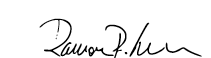
\includegraphics[width=65mm]{figs/logo/assinatura-ramon.png} \\[-4mm]
  \rule[2mm]{70mm}{0.1mm} \\
  \ramon \\[1mm]
  Coordenador do Projeto \\
}

%---------------------------------------------------------------------
\fim
 

\subsection{Setembro/2015}
  \subsubsection{Minuta de reunião (02-Setembro-2015)}

\begin{tabbing}
  Local \= xxx \kill
  Local \> : LEAD \\
  Data  \> : 02 de Setembro de 2015 \\
  Hora  \> : 13:00
\end{tabbing}

%---------------------------------------------------------------------
\participantes{
  \alana
  \gabriel,
  \julia,
  \estevão,
  \elael,
  \renan,
  \ramon.

}

\textbf{Aprovação da minuta}

\textbf{Update semanal do Projeto EMMA}
   							
\textbf{\alana.} 
	\begin{itemize}
		\item \textbf{Tarefas concluídas:}
			\begin{itemize}    
				\item Viagem Jirau.
				\item Relatório Auditoria.
			\end{itemize}
		
		\item \textbf{Novas tarefas:}
			\begin{itemize} 
				\item Ofício Viagem Jirau: passagens, diárias e locação de carros.
				\item Cronograma de viagem.
				\item Justificativa Ramon.
			\end{itemize}
	\end{itemize}   		
						
\textbf{\gabriel.} 
	\begin{itemize}
			\item Incluiu novas cotações para sensores Leica
			\item Implementou driver ROS para ROCK no Laser Scan.
			\end{itemize}
		
		\item \textbf{Novas tarefas:}
			\begin{itemize} 
				\item Continuar Point Cloud Alignment.
				\item Apresentação sobre alinhamento de pás e braço mecânico.
			\end{itemize}

					
			
   \textbf{\estevão.} 
	\begin{itemize}
		\item \textbf{Tarefas concluídas:}
			\begin{itemize}  
			  \item Contratou serviço para maquete, prazo de entrega de um mês.
			  \item Apresentação de Base de com trilho e suporte.
			\end{itemize}
		
		\item \textbf{Novas tarefas:}
			\begin{itemize} 
				\item Estado da arte de soluções modulares para bases robóticas em ambientes de difícil acesso.
			\end{itemize}
	\end{itemize}

	  \textbf{\renan.} 
	\begin{itemize}
		\item \textbf{Tarefas concluídas:}
			\begin{itemize}    
				\item Apresentou a aplicação de hardcoating Frame by Frame no OpenRave. 
				\item Estudo aproximando e afastando o robô da pá, na base criada por
				Estevão.
				\item Apresentou o início da pesquisa Dinâmica,
			\end{itemize}
		
		\item \textbf{Novas tarefas:}
			\begin{itemize} 
			    \item Continuar com estudo de Dinâmica
			\end{itemize}
	\end{itemize}	
	
	
	  \textbf{\elael.} 
	\begin{itemize}
		\item \textbf{Tarefas concluídas:}
			\begin{itemize}    
				\item Cotações para Point Laser. 
			\end{itemize}
		
		\item \textbf{Novas tarefas:}
			\begin{itemize} 
			    \item Continuar estudo de alinhamento de Point Cloud.
			\end{itemize}
	\end{itemize}			
			
			
   \textbf{\julia.} 
	\begin{itemize}
		\item \textbf{Tarefas concluídas:}
			\begin{itemize}    
				\item Apresentação processo de trablho para EMMA Fase 1: Descoberta para o
				time.
			\end{itemize}
		
		\item \textbf{Novas tarefas:}
			\begin{itemize} 

			    \item Apresentar Fase 2: Design.
			\end{itemize}
	\end{itemize}		



\textbf{Agenda para a próxima reunião:}
  \begin{itemize}
    \item Resultado de pesquisas individuais.
    \item Novas tarefas \& recomendações.
  \end{itemize}


\vspace{5mm}%
\parbox[t]{70mm}{
  Aprovado por: \\[5mm]
  \centering
  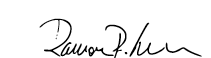
\includegraphics[width=65mm]{figs/logo/assinatura-ramon.png} \\[-4mm]
  \rule[2mm]{70mm}{0.1mm} \\
  \ramon \\[1mm]
  Coordenador do Projeto \\
}

%---------------------------------------------------------------------
\fim
   \subsubsection{Minuta de reunião (09-Setembro-2015)}

\begin{tabbing}
  Local \= xxx \kill
  Local \> : LEAD \\
  Data  \> : 09 de Setembro de 2015 \\
  Hora  \> : 13:00
\end{tabbing}

%---------------------------------------------------------------------
\participantes{
  \alana
  \gabriel,
  \julia,
  \estevão,
  \elael,
  \renan,
  \ramon.

}

\textbf{Aprovação da minuta}

\textbf{Update semanal do Projeto EMMA}
   							
\textbf{\alana.} 
	\begin{itemize}
		\item \textbf{Tarefas concluídas:}
			\begin{itemize}    
				\item Ofício Viagem Jirau: passagens, diárias e locação de carros.
				\item Cronograma de viagem.
				\item Justificativa Ramon.
			\end{itemize}
		
		\item \textbf{Novas tarefas:}
			\begin{itemize} 
				\item Coordenar com Gizele (ESBR) detalhes da viagem.
			\end{itemize}
	\end{itemize}   		
						
\textbf{\gabriel.} 
	\begin{itemize}
			\item Trabalhou no alinhamento da nuvem de pontos.
			\item Fez estudo sobre alinhamento de pás e braço mecânico para auxiliar o
			trabalho de dinâmica do Renan.
			\end{itemize}
		
		\item \textbf{Novas tarefas:}
			\begin{itemize} 
				\item Continuar trabalhando com alinhamento de point cloud. Cruzamento de
				modelos e informações diferentes que possam satisfazer provar a viabilidade
				de sensores na atividade de calibração.
			\end{itemize}

					
			
   \textbf{\estevão.} 
	\begin{itemize}
		\item \textbf{Tarefas concluídas:}
			\begin{itemize}  
			  \item Apresentação de possíveis soluções modulares para bases robóticas em
			  ambientes de difícil acesso.
			\end{itemize}
		
		\item \textbf{Novas tarefas:}
			\begin{itemize} 
				\item Continuar estudo de bases e sua logística em ambientes confinados.
			\end{itemize}
	\end{itemize}

	  \textbf{\renan.} 
	\begin{itemize}
		\item \textbf{Tarefas concluídas:}
			\begin{itemize}    
				\item Continuou apresentação do estudo de dinâmica.
			\end{itemize}
		
		\item \textbf{Novas tarefas:}
			\begin{itemize} 
			    \item Adicionar um estudo de discretizaçào da pá.
			\end{itemize}
	\end{itemize}	
	
	
	  \textbf{\elael.} 
	\begin{itemize}
		\item \textbf{Tarefas concluídas:}
			\begin{itemize}    
				\item Reuniu elementos apra apresentação em Jirau antes de sair de férias.
			\end{itemize}
		
			
   \textbf{\julia.} 
	\begin{itemize}
		\item \textbf{Tarefas concluídas:}
			\begin{itemize}    
				\item Apresentação processo de trabalho para EMMA Fase 2: Design.
				\item Coordenar material para apresentações em Jirau.
			\end{itemize}
		
		\item \textbf{Novas tarefas:}
			\begin{itemize} 

			    \item Apresentar Fase 3: Desenvolvimento.
			\end{itemize}
	\end{itemize}		



\textbf{Agenda para a próxima reunião:}
  \begin{itemize}
    \item Resultado de pesquisas individuais.
    \item Novas tarefas \& recomendações.
  \end{itemize}


\vspace{5mm}%
\parbox[t]{70mm}{
  Aprovado por: \\[5mm]
  \centering
  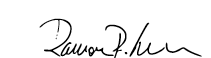
\includegraphics[width=65mm]{figs/logo/assinatura-ramon.png} \\[-4mm]
  \rule[2mm]{70mm}{0.1mm} \\
  \ramon \\[1mm]
  Coordenador do Projeto \\
}

%---------------------------------------------------------------------
\fim
   \subsubsection{Minuta de reunião (16-Setembro-2015)}

\begin{tabbing}
  Local \= xxx \kill
  Local \> : LEAD \\
  Data  \> : 16 de Setembro de 2015 \\
  Hora  \> : 13:00
\end{tabbing}

%---------------------------------------------------------------------
\participantes{
  \gabriel,
  \julia,
  \estevão,
  \renan,
  \ramon.
 
}

\textbf{Aprovação da minuta}

\textbf{Update semanal do Projeto EMMA}
   							
							
\textbf{\gabriel.} 
	\begin{itemize}
			\item Continuou trabalhando com alinhamento de point cloud. Cruzamento de
			modelos e informações diferentes que possam satisfazer provar a viabilidade de sensores na atividade de calibração.
			\item Separou material para apresentação de Jirau antes de sair de férias.
			\end{itemize}
					
			
   \textbf{\estevão.} 
	\begin{itemize}
		\item \textbf{Tarefas concluídas:}
			\begin{itemize}  
			  \item Adicionou desenhos de solidWorks ao estudos de bases em ambientes
			  confinados.
			  \item Logística e pagamento da maquete 5:1.
			\end{itemize}
		
		\item \textbf{Novas tarefas:}
			\begin{itemize} 
				\item Definir material para apresentação de Jirau.
				\item Novo conceito de base com um DOF a mais para o Motoman MH12.
			\end{itemize}
	\end{itemize}

	  \textbf{\renan.} 
	\begin{itemize}
		\item \textbf{Tarefas concluídas:}
			\begin{itemize}    
				\item Estudo de discretização da pá.
			\end{itemize}
		
		\item \textbf{Novas tarefas:}
			\begin{itemize} 
			    \item Tradução do SOTA.
			    \item Pesquisar velocidades analíticas do braço usando as normais da pá.
			\end{itemize}
	\end{itemize}	
	
		
			
   \textbf{\julia.} 
	\begin{itemize}
		\item \textbf{Tarefas concluídas:}
			\begin{itemize}    
				\item Apresentou Proposta de Mestrado.
			\end{itemize}
		
		\item \textbf{Novas tarefas:}
			\begin{itemize} 
			    \item Apresentar Fase 3: Desenvolvimento. 
			\end{itemize}
	\end{itemize}		



\textbf{Agenda para a próxima reunião:}
  \begin{itemize}
    \item Resultado de pesquisas individuais.
    \item Novas tarefas \& recomendações.
  \end{itemize}


\vspace{5mm}%
\parbox[t]{70mm}{
  Aprovado por: \\[5mm]
  \centering
  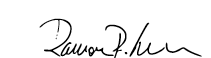
\includegraphics[width=65mm]{figs/logo/assinatura-ramon.png} \\[-4mm]
  \rule[2mm]{70mm}{0.1mm} \\
  \ramon \\[1mm]
  Coordenador do Projeto \\
}

%---------------------------------------------------------------------
\fim   
   \subsubsection{Minuta de reunião (24-Setembro-2015)}

\begin{tabbing}
  Local \= xxx \kill
  Local \> : LEAD \\
  Data  \> : 24 de Setembro de 2015 \\
  Hora  \> : 13:00
\end{tabbing}

%---------------------------------------------------------------------
\participantes{
  \alana
  \julia,
  \elael,
  \estevão,
  \renan,
  \ramon.

}

\textbf{Aprovação da minuta}

\textbf{Update semanal do Projeto EMMA}
   							
\textbf{\alana.} 
	\begin{itemize}
		\item \textbf{Tarefas concluídas:}
			\begin{itemize}    
				\item Cronograma de viagem.
				\item Administrativo Coppetec
				\item Justificativa Ramon
				 
			\end{itemize}
		
		\item \textbf{Novas tarefas:}
			\begin{itemize} 
				\item Prestação de Contas
			\end{itemize}
	\end{itemize}   		

	  \textbf{\renan.} 
	\begin{itemize}
		\item \textbf{Tarefas concluídas:}
			\begin{itemize}    
				\item Apresentou sobre dinâmica com braços robóticos.
			\end{itemize}
		
		\item \textbf{Novas tarefas:}
			\begin{itemize} 
			    \item Fazer melhor discretização.
			    \item Velocidades analítica do braço usando as normais da pá.
			    \item Ver com Ramon dinâmica em outros ambientes da pá.
			\end{itemize}
	\end{itemize}	
	 
	
   \textbf{\julia.} 
	\begin{itemize}
		\item \textbf{Tarefas concluídas:}
			\begin{itemize}    
				\item Apresentação processo de trabalho para EMMA Fase 3: Desenvolvimento.
				\item Discutiu com o time os aspectos importantes do desenvolvimento do
				produto e seu escopo. 
			\end{itemize}
		
		\item \textbf{Novas tarefas:}
			\begin{itemize} 
			    \item Questionário para o escopo do produto EMMA.
			    \item Organizar apresentação de JIRAU.
			\end{itemize}
	\end{itemize}		



\textbf{Agenda para a próxima reunião:}
  \begin{itemize}
    \item Resultado de pesquisas individuais.
    \item Novas tarefas \& recomendações.
  \end{itemize}


\vspace{5mm}%
\parbox[t]{70mm}{
  Aprovado por: \\[5mm]
  \centering
  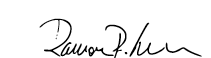
\includegraphics[width=65mm]{figs/logo/assinatura-ramon.png} \\[-4mm]
  \rule[2mm]{70mm}{0.1mm} \\
  \ramon \\[1mm]
  Coordenador do Projeto \\
}

%---------------------------------------------------------------------
\fim 
 
\subsection{Outubro/2015}
  \subsubsection{Minuta de reunião (01-Outubro-2015)}

\begin{tabbing}
  Local \= xxx \kill
  Local \> : LEAD \\
  Data  \> : 01 de Outubro de 2015 \\
  Hora  \> : 13:00
\end{tabbing}

%---------------------------------------------------------------------
\participantes{
  \alana
  \julia,
  \elael,
  \estevão,
  \renan,
  \ramon.

}

\textbf{Aprovação da minuta}

\textbf{Update semanal do Projeto EMMA}
   							
\textbf{\alana.} 
	\begin{itemize}
		\item \textbf{Tarefas concluídas:}
			\begin{itemize}    
				\item Viagem Jirau Outubro: passagens, aluguel de carro e diárias.

			 
			\end{itemize}
		
		\item \textbf{Novas tarefas:}
			\begin{itemize} 
				\item Prestação de Contas com Gizele em 20 de Outubro.
			\end{itemize}
	\end{itemize}   		

	  \textbf{\renan.} 
	\begin{itemize}
		\item \textbf{Tarefas concluídas:}
			\begin{itemize}    
				\item Aprimorou a discretização de pás.
				\item Estudo sobre velocidade analítica da pá.
			\end{itemize}
		
		\item \textbf{Novas tarefas:}
			\begin{itemize} 
			    \item Ver dinâmica em outros ambientes de simulação.
			    \item Tradução SOTA.
			\end{itemize}
	\end{itemize}	
	
	
   \textbf{\julia.} 
	\begin{itemize}
		\item \textbf{Tarefas concluídas:}
			\begin{itemize}    
				\item Apresentação Jirau, material de todas as pesquisas coordenado.
				em uma só apresentação.
				\item Questionários técnicos para escopo do produto EMMA.
			\end{itemize}
		
		\item \textbf{Novas tarefas:}
			\begin{itemize} 
			    \item Requesitos funcionais e não funcionais do software.
			    \item Organizar apresentação de JIRAU.
			\end{itemize}
	\end{itemize}		



\textbf{Agenda para a próxima reunião:}
  \begin{itemize}
    \item Resultado de pesquisas individuais.
    \item Novas tarefas \& recomendações.
  \end{itemize}


\vspace{5mm}%
\parbox[t]{70mm}{
  Aprovado por: \\[5mm]
  \centering
  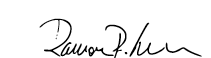
\includegraphics[width=65mm]{figs/logo/assinatura-ramon.png} \\[-4mm]
  \rule[2mm]{70mm}{0.1mm} \\
  \ramon \\[1mm]
  Coordenador do Projeto \\
}

%---------------------------------------------------------------------
\fim
  \subsubsection{Minuta de reunião (31-Outubro-2015)}

\begin{tabbing}
  Local \= xxx \kill
  Local \> : LEAD \\
  Data  \> : 31 de Outubro de 2015 \\
  Hora  \> : 13:00
\end{tabbing} 

%---------------------------------------------------------------------
\participantes{
  \gabriel,
  \julia,
  \estevão,
  \elael,
  \ramon.

}

\textbf{Aprovação da minuta}

\textbf{Update semanal do Projeto EMMA}
   									
						
\textbf{\gabriel.} 
	\begin{itemize}
			\item Iniciou o processo de compras para Sensor de scaneamento de
			ambiente.
			\item Estudo sobre localização de objetos com PCL. Encontrou Dataset com
			modelos compatíveis.
			\end{itemize}
		
		\item \textbf{Novas tarefas:}
			\begin{itemize} 
				\item Estudo sobre 'welding'. Laboratórios na UFRJ que façam pesquisa na
				área.
				\item Teste utilizando imagem de 'point cloud' gerada pelo sensor da Faro
				durante o teste em Jirau.
			\end{itemize}

					
			
   \textbf{\estevão.} 
	\begin{itemize}
		\item \textbf{Tarefas concluídas:}
			\begin{itemize}    
			    \item Desenho do último conceito de base proposto.
				\item Orçamento do Motoman, perguntas de volta aos fornecedores.
				\item Maquete 1:1 com professor da UFRJ.
				
			\end{itemize}
		
		\item \textbf{Novas tarefas:}
			\begin{itemize} 
			    \item Formalizar último conceito de base.
			    \item Repassar possibilidadepara customização do Modelo de Motoman que
			    queremos.
			\end{itemize}
	\end{itemize}

	
	  \textbf{\elael.} 
	\begin{itemize}
		\item \textbf{Tarefas concluídas:}
			\begin{itemize}    
				\item Relatório técnico do teste da Faro.
			\end{itemize}
		
		\item \textbf{Novas tarefas:}
			\begin{itemize} 
			    \item Estudo sobre 'Griding'. Pesquisar laboratórios na UFRJ que façam esse
				tipo de pesquisa.
			\end{itemize}
	\end{itemize}			
			
			
   \textbf{\julia.} 
	\begin{itemize}
		\item \textbf{Tarefas concluídas:}
			\begin{itemize}    
				\item Estruturar análise de tarefas com o processo de Calibração.
				\item Relatórios de Viagem.
			\end{itemize}
		
		\item \textbf{Novas tarefas:}
			\begin{itemize} 
			    \item Apresentação para time
			\end{itemize}
	\end{itemize}		



\textbf{Agenda para a próxima reunião:}
  \begin{itemize}
    \item Resultado de pesquisas individuais.
    \item Novas tarefas \& recomendações.
  \end{itemize}


\vspace{5mm}%
\parbox[t]{70mm}{
  Aprovado por: \\[5mm]
  \centering
  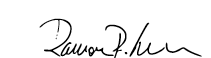
\includegraphics[width=65mm]{figs/logo/assinatura-ramon.png} \\[-4mm]
  \rule[2mm]{70mm}{0.1mm} \\
  \ramon \\[1mm]
  Coordenador do Projeto \\
}

%---------------------------------------------------------------------
\fim 

\subsection{Novembro/2015}
  \subsubsection{Minuta de reunião (05-Novembro-2015)}

\begin{tabbing}
  Local \= xxx \kill
  Local \> : LEAD \\
  Data  \> : 05 de Novembro de 2015 \\
  Hora  \> : 13:00
\end{tabbing} 

%---------------------------------------------------------------------
\participantes{
  \gabriel,
  \julia,
  \estevão,
  \elael,
  \renan,
  \ramon.

}

\textbf{Aprovação da minuta}

\textbf{Update semanal do Projeto EMMA}
   									
						
\textbf{\gabriel.} 
	\begin{itemize}
			\item Agilizar a compra do sensor da Faro.
			\item Trabalho em andamento do com Point Cloud e PCL.
			\end{itemize}
		
		\item \textbf{Novas tarefas:}
			\begin{itemize} 
				\item Entrar em contato com laboratório da UFRJ que está fazendo trabalho
				com 'welding'.
			\end{itemize}

					
			
   \textbf{\estevão.} 
	\begin{itemize}
		\item \textbf{Tarefas concluídas:}
			\begin{itemize}    
			    \item Formalizou modificações do conceito de base para escotilha
			    inferior, previsto na última reunião.
				
			\end{itemize}
		
		\item \textbf{Novas tarefas:}
			\begin{itemize} 
			    \item Agilizar a compra de Motoman, entrar em contato e verificar
			    se configuração que queremos é possível.
			    \item Formalizar conceito no Journal do EMMA.
			\end{itemize}
	\end{itemize}

	
	  \textbf{\elael.} 
	\begin{itemize}
		\item \textbf{Tarefas concluídas:}
			\begin{itemize}    
				\item Relatório técnico do teste do sensor da Faro.
				\item Entrar em contato com laboratório da UFRJ que está fazendo trabalho
				com 'griding'.
			\end{itemize}
		
		\item \textbf{Novas tarefas:}
			\begin{itemize} 
			    \item Formalizar descobertas do teste de sensores no Journal do EMMA.
			\end{itemize}
	\end{itemize}			
			
  \textbf{\renan.} 
	\begin{itemize}
		\item \textbf{Tarefas concluídas:}
			\begin{itemize}    
				\item Trabalhando no modelo de pá gerada através do point cloud do sensor da
				Faro.
			\end{itemize}
		
		\item \textbf{Novas tarefas:}
			\begin{itemize} 
			    \item Formalizar descobertas do teste de sensores no Journal do EMMA.
			\end{itemize}
	\end{itemize}	
			
   \textbf{\julia.} 
	\begin{itemize}
		\item \textbf{Tarefas concluídas:}
			\begin{itemize}    
				\item Análise de Tarefas da Calibração.
				\item Estudo de processos que podem ser aplicados na construção do software,
				possíveis problemas e possibilidades de arquitetura de informação.
			\end{itemize}
		
		\item \textbf{Novas tarefas:}
			\begin{itemize} 
			    \item Possibilidades para análise de tarefas de outras atividades
			    (hardcoating e planejamento de trajetória).
			\end{itemize}
	\end{itemize}		



\textbf{Agenda para a próxima reunião:}
  \begin{itemize}
    \item Resultado de pesquisas individuais.
    \item Novas tarefas \& recomendações.
  \end{itemize}


\vspace{5mm}%
\parbox[t]{70mm}{
  Aprovado por: \\[5mm]
  \centering
  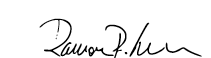
\includegraphics[width=65mm]{figs/logo/assinatura-ramon.png} \\[-4mm]
  \rule[2mm]{70mm}{0.1mm} \\
  \ramon \\[1mm]
  Coordenador do Projeto \\
}

%---------------------------------------------------------------------
\fim
  \subsubsection{Minuta de reunião (12-Novembro-2015)}

\begin{tabbing}
  Local \= xxx \kill
  Local \> : LEAD \\
  Data  \> : 12 de Novembro de 2015 \\
  Hora  \> : 13:00
\end{tabbing} 

%---------------------------------------------------------------------
\participantes{
  \gabriel,
  \julia,
  \estevão,
  \elael,
  \renan,
  \ramon.

}

\textbf{Aprovação da minuta}

\textbf{Update semanal do Projeto EMMA} 

\text {Objetivo para conclusão da viabilidade técnica}
   									
					
		
		\item \textbf{Pá 1:1}
			\begin{itemize} 
			    \item Design e construção.
			\end{itemize}
			
		\item \textbf{Manipulador}
			\begin{itemize} 
			    \item Definir controle através do ROSS ou do ROCK.
			    \item Telemetria
			    \item Software: Move it ou Planning
			\end{itemize}	

		\item \textbf{Pintura\Coating}
			\begin{itemize} 
			    \item Definir 'end effector' que fará a simulação do 'coating'.
			\end{itemize}	
		
		\item \textbf{Scanner}
			\begin{itemize} 
			    \item Extrair dados da pá para  ROCK e para o ROSS.
			    \item Alinhamento das medidas dos modelos extraídos com oclusão.
			    \item Dados do braço robótico.
			    \item Teste de calibração esquematizado.
			\end{itemize}
			
				
\item \textbf{Requisitos para espaço destinado a teste}
			\begin{itemize} 
			    \item Preço estimado para:
			    \item Pá (estevão)
			    \item manipulador (orçamento)
				\item pistola de tinta (Pedro 1 estagiário)
				\item trilhos (estevão)
				\item scanner (gabriel)
				\item base (estevão)
				\item infraestrutura
   				\item restrições apresentar projeto para arquiteta da Coppe
   			\end{itemize}	




\textbf{Agenda para a próxima reunião:}
  \begin{itemize}
    \item Resultado de pesquisas individuais.
    \item Novas tarefas \& recomendações.
  \end{itemize}


\vspace{5mm}%
\parbox[t]{70mm}{
  Aprovado por: \\[5mm]
  \centering
  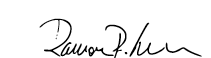
\includegraphics[width=65mm]{figs/logo/assinatura-ramon.png} \\[-4mm]
  \rule[2mm]{70mm}{0.1mm} \\
  \ramon \\[1mm]
  Coordenador do Projeto \\
}

%---------------------------------------------------------------------
\fim 

\subsection{Dezembro/2015}
  \subsubsection{Minuta de reunião (03-Dezembro-2015)}

\begin{tabbing}
  Local \= xxx \kill
  Local \> : LEAD \\
  Data  \> : 03 de Dezembro de 2015 \\
  Hora  \> : 13:00
\end{tabbing} 

%---------------------------------------------------------------------
\participantes{
  \gabriel,
  \julia,
  \estevão,
  \elael,
  \renan,
  \ramon.

}

\textbf{Aprovação da minuta}

\textbf{Update semanal do Projeto EMMA}
   									
						
	\begin{itemize}
			\item Trabalho de pesquisa interrompido para o a execução de relatório da
			ESBR para a ANEEL.
			\end{itemize}
		
					
			

\textbf{Agenda para a próxima reunião:}
  \begin{itemize}
    \item Resultado de pesquisas individuais.
    \item Novas tarefas \& recomendações.
  \end{itemize}


\vspace{5mm}%
\parbox[t]{70mm}{
  Aprovado por: \\[5mm]
  \centering
  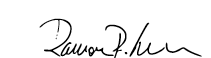
\includegraphics[width=65mm]{figs/logo/assinatura-ramon.png} \\[-4mm]
  \rule[2mm]{70mm}{0.1mm} \\
  \ramon \\[1mm]
  Coordenador do Projeto \\
}

%---------------------------------------------------------------------
\fim
  \subsubsection{Minuta de reunião (10-Dezembro-2015)}

\begin{tabbing}
  Local \= xxx \kill
  Local \> : LEAD \\
  Data  \> : 10 de Dezembro de 2015 \\
  Hora  \> : 10:00
\end{tabbing} 

%---------------------------------------------------------------------
\participantes{
  \gabriel,
  \julia,
  \estevão,
  \elael,
  \renan,
  \ramon.

}

\textbf{Aprovação da minuta}

\textbf{Update semanal do Projeto EMMA}
   									
						
\textbf{\gabriel.} 
	\begin{itemize}
			\item Compra do Sensor a laser da empesa Faro enviada.
			\end{itemize}
		
		\item \textbf{Novas tarefas:}
			\begin{itemize} 
				\item Trabalho em andamento do com Point Cloud e PCL.
				\item Pesquisou possibilidade para 'oclusão'.
			\end{itemize}

					
   \textbf{\estevão.} 
	\begin{itemize}
		\item \textbf{Tarefas concluídas:}
			\begin{itemize}    
			    \item Definiu aspectos técnicos para a cotação do braço mecânico
			    Motoman MH12.
			    \item Coloborou com Renan para estudos de simulações.
				
			\end{itemize}
		
		\item \textbf{Novas tarefas:}
			\begin{itemize} 
			    \item Ajustes no desenho da base.
			\end{itemize}
	\end{itemize}

	
	  \textbf{\elael.} 
	\begin{itemize}
		\item \textbf{Tarefas concluídas:}
			\begin{itemize}    
				\item Pesquisa bibliográfica para o segundo artigo do
				EMMA-DETAIL: Estudo do conceito para metodologia e revestimento robótico
de turbinas.
			\end{itemize}
		
		\item \textbf{Novas tarefas:}
			\begin{itemize} 
			    \item Dar início ao segundo artigo do EMMA-DETAIL, Estudo do conceito para metodologia e revestimento robótico
de turbinas.
			\end{itemize}
	\end{itemize}			
			
  \textbf{\renan.} 
	\begin{itemize}
		\item \textbf{Tarefas concluídas:}
			\begin{itemize}    
				\item Executou diferentes simulações nos softwares MoveIt e no OpenRave.
			\end{itemize}
		
		\item \textbf{Novas tarefas:}
			\begin{itemize} 
			    \item Formalizar simulações em um relatório.
			\end{itemize}
	\end{itemize}	
			
   \textbf{\julia.} 
	\begin{itemize}
		\item \textbf{Tarefas concluídas:}
			\begin{itemize}    
				\item Descrição de tarefas: calibração, planejamento de trajetória e metalização para artigo.
				\item Cobrar testes do grupo formado para questionários da pesquisa.
			\end{itemize}
		
		\item \textbf{Novas tarefas:}
			\begin{itemize} 
			    \item Formato de artigo para interface de usuário EMMA.
			\end{itemize}
	\end{itemize}		



\textbf{Agenda para a próxima reunião:}
  \begin{itemize}
    \item Resultado de pesquisas individuais.
    \item Novas tarefas \& recomendações.
  \end{itemize}


\vspace{5mm}%
\parbox[t]{70mm}{
  Aprovado por: \\[5mm]
  \centering
  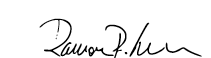
\includegraphics[width=65mm]{figs/logo/assinatura-ramon.png} \\[-4mm]
  \rule[2mm]{70mm}{0.1mm} \\
  \ramon \\[1mm]
  Coordenador do Projeto \\
}

%---------------------------------------------------------------------
\fim    

\subsection{Janeiro/2016} 
  \subsubsection{Minuta de reunião (07-Janeiro-2016)}

\begin{tabbing}
  Local \= xxx \kill
  Local \> : LEAD \\
  Data  \> : 07 de Janeiro de 2016 \\
  Hora  \> : 10:00
\end{tabbing} 

%---------------------------------------------------------------------
\participantes{
  \gabriel,
  \julia,
  \estevão,
  \elael,
  \renan,
  \ramon.

}

\textbf{Aprovação da minuta}

\textbf{Update semanal do Projeto EMMA}

\begin{itemize}
			\item Definir datas e entregáveis para o final do EMMA com ESBR.
			\item Feedback RIJEZA para válvula.
			\end{itemize}
   									
						
\textbf{\gabriel.} 
	\begin{itemize}
			\item Pesquisa ‘Oclusão’: encontrou simulador de laser scan para criar cenas
			de oclusão e testas algorítmos.
			\end{itemize}
		
		\item \textbf{Novas tarefas:}
			\begin{itemize} 
				\item Trabalho em andamento do com Nuvem de Pontos e PCL.
			\end{itemize}

					
   \textbf{\estevão.} 
	\begin{itemize}
		\item \textbf{Tarefas concluídas:}
			\begin{itemize}    
			    \item Adicionar grau de liberdade em Y na base.
			    \item Cotação Motoman encaminhada.
				
			\end{itemize}
		
		\item \textbf{Novas tarefas:}
			\begin{itemize} 
			    \item Desenhar ambiente com 5 pás da Usina Santo Antônio.
			    \item Retomar com RIJEZA o projeto da válvula, vai preparar um diagrama
			    explicativo com o conceito da solução.
			\end{itemize}
	\end{itemize}

	
	  \textbf{\elael.} 
	\begin{itemize}
		\item \textbf{Tarefas concluídas:}
			\begin{itemize}    
				\item Artigo de detalhamento EMMA-DETAIL, o Estudo de viabilidade técnica
				para revestimento robótico de turbinas: organizou conteúdo e estrutura, re-leu os
				artigos anteriores e terminou introdução.
			\end{itemize}
		
		\item \textbf{Novas tarefas:}
			\begin{itemize} 
			    \item Dar continuidade ao artigo do EMMA-DETAIL, o Estudo de viabilidade
			    técnica para revestimento robótico de turbinas.
			\end{itemize}
	\end{itemize}			
			
  \textbf{\renan.} 
	\begin{itemize}
		\item \textbf{Tarefas concluídas:}
			\begin{itemize}    
				\item Relatório de simulações dos softwares Open Rave e MoveIt.
			\end{itemize}
		
		\item \textbf{Novas tarefas:}
			\begin{itemize} 
			    \item Ver revisão de artigo com Ramon.
			\end{itemize}
	\end{itemize}	
			
   \textbf{\julia.} 
	\begin{itemize}
		\item \textbf{Tarefas concluídas:}
			\begin{itemize}    
				\item Conteúdo para artigo para Interface de usuário EMMA.
				\item cobrar testes do grupo formado para questionários da pesquisa.
			\end{itemize}
		
		\item \textbf{Novas tarefas:}
			\begin{itemize} 
			    \item Resultados de questionários.
			    \item Formato de artigo conferido por Ramon.
			\end{itemize}
	\end{itemize}		



\textbf{Agenda para a próxima reunião:}
  \begin{itemize}
    \item Resultado de pesquisas individuais.
    \item Novas tarefas \& recomendações.
  \end{itemize}


\vspace{5mm}%
\parbox[t]{70mm}{
  Aprovado por: \\[5mm]
  \centering
  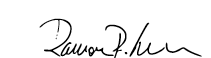
\includegraphics[width=65mm]{figs/logo/assinatura-ramon.png} \\[-4mm]
  \rule[2mm]{70mm}{0.1mm} \\
  \ramon \\[1mm]
  Coordenador do Projeto \\
}

%---------------------------------------------------------------------
\fim
  \subsubsection{Minuta de reunião (27-Janeiro-2016)}

\begin{tabbing}
  Local \= xxx \kill
  Local \> : LEAD \\
  Data  \> : 27 de Janeiro de 2016 \\
  Hora  \> : 10:00
\end{tabbing} 

%---------------------------------------------------------------------
\participantes{
  \gabriel,
  \julia,
  \estevão,
  \elael,
  \renan,
  \ramon.

}

\textbf{Aprovação da minuta}

\textbf{Update semanal do Projeto EMMA}

						
\textbf{\gabriel.} 
	\begin{itemize}
			\item Relatório de localização da pá.
			\item Implementação de verificação de hipóteses de modelos encontrados.
			\end{itemize}
		
		\item \textbf{Novas tarefas:}
			\begin{itemize} 
				\item Implementar localização da pá no framework a ser utilizado no robô.
			\end{itemize}

					
   \textbf{\estevão.} 
	\begin{itemize}
		\item \textbf{Tarefas concluídas:}
			\begin{itemize}    
			    \item Conjunto de peças do trilho.
			    \item Reunião Bosch.
			    \item Definir peças a serem compradas no Brasil.
				
			\end{itemize}
		
		\item \textbf{Novas tarefas:}
			\begin{itemize} 
			    \item Rotação e elevação da base.
			\end{itemize}
	\end{itemize}

	
	  \textbf{\elael.} 
	\begin{itemize}
		\item \textbf{Tarefas concluídas:}
			\begin{itemize}    
				\item Enviou motivação, objetivos e metodologia para o orientador.
			\end{itemize}
		
		\item \textbf{Novas tarefas:}
			\begin{itemize} 
			    \item Revisão bibliográfica do Mestrado.
			    \item Verificação de trajetória.(c/ Renan)
			    \item Localização (c/ gabriel)
			\end{itemize}
	\end{itemize}			
			
  \textbf{\renan.} 
	\begin{itemize}
		\item \textbf{Tarefas concluídas:}
			\begin{itemize}    
				\item Estudo de artigos de planejamento de trajetória.
				\item Estudo da Tese do Pal.
				\item Formalização do problema.
			\end{itemize}
		
		\item \textbf{Novas tarefas:}
			\begin{itemize} 
			    \item Estudo dos Jacobianos nos pontos da pá.
			    \item Otimização dos ângulos das juntas para minimizar o torque.
			\end{itemize}
	\end{itemize}	
			
   \textbf{\julia.} 
	\begin{itemize}
		\item \textbf{Tarefas concluídas:}
			\begin{itemize}    
				\item Relatorio: Fluxogramade tarefas, diagrama de casos de uso, perfil de
				usuários.
				\item Adicionar relatório ao EMMA-DETAIL.
			\end{itemize}
		
		\item \textbf{Novas tarefas:}
			\begin{itemize} 
			    \item Resultados de questionários para concluir pesquisa do usuário.
			    \item Adicionar formulários de casos de uso ao EMMA DETAIL.
			\end{itemize}
	\end{itemize}		



\textbf{Agenda para a próxima reunião:}
  \begin{itemize}
    \item Resultado de pesquisas individuais.
    \item Novas tarefas \& recomendações.
  \end{itemize}


\vspace{5mm}%
\parbox[t]{70mm}{
  Aprovado por: \\[5mm]
  \centering
  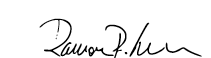
\includegraphics[width=65mm]{figs/logo/assinatura-ramon.png} \\[-4mm]
  \rule[2mm]{70mm}{0.1mm} \\
  \ramon \\[1mm]
  Coordenador do Projeto \\
}

%---------------------------------------------------------------------
\fim    
%---------------------------------------------------------------------

%---------------------------------------------------------------------
\end{document}

